\documentclass[12pt, a4paper]{report}
\usepackage{tbagrelstandard}
\usepackage{charter}
\usepackage{lastpage}
\usepackage{indentfirst}
\usepackage{marvosym}

\usepackage[bibstyle=numeric, sorting=none]{biblatex}
\bibliography{biblio}
\renewcommand{\bibfont}{\small}

%\setlength{\parskip}{\baselineskip}

\title{
\sc{\bf{{\LARGE Travaux~$\cdot$~Personnels $\cdot$~Encadrés}}}\\
\vspace{1cm}
{\itshape{\Large Première Scientifique}} \\
\vspace{1cm}
\ovalbox{\parbox[c][2.5cm][c]{0.65\textwidth}{
\begin{center}
\sc{\bf{\Large - L'insolite -\\}}
\sc{\bf{\Large La réalité virtuelle}}
\end{center}}}}

\newcommand{\rendulien}[1]{{\normalfont\tt{#1}}}


\newcommand{\euro}{\,\EUR}
\renewcommand{\headrulewidth}{0.5pt}
\renewcommand{\footrulewidth}{0.5pt}

\fancyhead[L]{\footnotesize \leftmark}%
\fancyhead[C]{\small \bf{\sc{tpe} - La réalité virtuelle}}%
\fancyhead[R]{\footnotesize \rightmark}%
\fancyfoot[L]{\footnotesize Lycée Arthur \sc{Varoquaux}}%
\fancyfoot[C]{\small Page \bf{\thepage} sur \bf{\pageref{LastPage}}}%
\fancyfoot[R]{\footnotesize 2017 - 2018}%

\fancypagestyle{plain}{%
\fancyhead[L]{\footnotesize \leftmark}%
\fancyhead[C]{\small \bf{\sc{tpe} - La réalité virtuelle}}%
\fancyhead[R]{\footnotesize \rightmark}%
\fancyfoot[L]{\footnotesize Lycée Arthur \sc{Varoquaux}}%
\fancyfoot[C]{\small Page \bf{\thepage} sur \bf{\pageref{LastPage}}}%
\fancyfoot[R]{\footnotesize 2017 - 2018}%
}

\author{
Lucie \sc{Chevallereau}
\\
Marie \sc{Bagrel}
\\
Nicolas \sc{Gobillard}
\\
\sc{ps1}
}
\date{\sc{Année} 2017 - 2018}

\begin{document}
\pagestyle{fancy}
\selectlanguage{french}

\vfill
\maketitle{}
\vfill

\newpage{}
\tableofcontents{}

\newpage{}
%%%%%%%%%%%%%%%%%%%%%%%%%%%%%%%%%%%%%%%%%%%%%%%%%%%%%%%%%%%%%%%%%%%%%%%%%%%%%%%

\section*{Introduction}

De nos jours, dans le domaine des jeux, les joueurs recherchent de plus en plus à se rapprocher de la réalité lorsqu'ils jouent pour leur donner une impression d'immersion la plus totale. Afin de répondre à cette volonté de réel, les ingénieurs ont crée les casques de réalité virtuelle comme l'Occulus Rift et bien d'autres.
Mais ces casques se sont vite répandus dans d'autres domaines comme le médical. La réalité virtuelle s'est aussi développée dans les domaines de la simulation dans l'aéronautique, l'aviation\ldots{}
Des études ont aussi été menées par les scientifiques sur les effets de cette nouvelle technologie, encore en plein développement.
Effectivement on constate chez certains individus des effets néfastes lors de l'utilisation.

\begin{quotation}\noindent\itshape
La réalité virtuelle, est-elle une révolution grâce à l'immersion ou un danger pour la santé ?
\end{quotation}


Pour tenter de répondre à cette question, nous allons d'abord définir ce qu'est la réalité virtuelle et analyser le fonctionnement de certains ancêtres du casque de réalité virtuelle. Puis dans une seconde partie, nous allons étudier le fonctionnement de l'\oe{}il et du cerveau. Ensuite, nous verrons comment fonctionne le casque HTC Vive  grâce à une expérience avec ce dernier. Nous aborderons ensuite les nombreuses innovations et modifications que la réalité virtuelle à permis dans de multiples domaines. Enfin nous parlerons des effets néfastes que cette immersion peut causer sur notre santé.


\part{Définition, fonctionnement et expériences}

\chapter[Réalité virtuelle]{Qu'est ce que la réalité virtuelle ?}

\section{Définition}

\paragraph{\'{E}tymologie}
Le mot réalité représente ce que l'on vit et ressent en tant qu'êtres humains
Le mot virtuel désigne une chose non physique, non réelle
La réalité virtuelle signifie donc  une expérience proche du réel avec une simulation de la réalité et une immersion importante

\paragraph{Définition générale}
La réalité virtuelle est un groupe de mots pour désigner une environnement en 3 dimensions généré par un ordinateur. La personne concernée devient un élément de l'environnement et a un sentiment d'immersion car elle peut manipuler des objets, réaliser des actions \ldots{}
Cette impression de réel est due aux informations données à nos sens qui modifient nos perceptions car c'est uniquement grâce à ces informations sensorielles que la réalité existe. Comme nos sens recoivent des informations, on a cette impression de réel. Ceci explique la notion de réalité virtuelle

\paragraph{Définition en markéting}
En marketing, le casque de réalité virtuelle est généralement utilisé pour mettre le consommateur en situation d'usage virtuel d'un produit ou service. En voici quelques exemples :\\
\begin{itemize}
\item En point de vente notamment pour présenter une gamme de produits occupant beaucoup d'espace : décathlon lance la réalité virtuelle pour visiter ses tentes familiales. A l'aide du casque Samsung Gear VR, les utilisateurs vont pouvoir visualiser les différents modèles de tentes, pour choisi celle qui leur convient le mieux.

\item Le Google cardboard a permis de faire visiter et tester virtuellement une voiture : la Volvo XC90. L'entreprise Volvo a fait un partenariat avec l'agence R/GA et les framestores.
\end{itemize}

\section[Historique]{Historique de la réalité virtuelle}

Les premières allusions à la réalité virtuelle sont dans la science-fiction. Comme la nouvelle  Pygmalion spectacles  de Stanley, G Weinbaum, publiée en 1935, où dans l'histoire, on évoque des lunettes capables de retranscrire les sensations, les sens : d'être en immersion totale dans la fiction.
\begin{center}
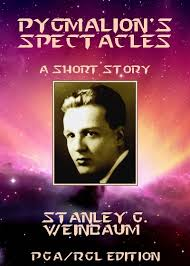
\includegraphics[scale=0.3]{pygmalion.jpeg}
\captionof{figure}{Couverture du livre \it{Pygmalion}\tss{\cite{pygmalion}}}
\end{center}



Un ancêtre de la réalité virtuelle est le View master, développé en 1940, un dispositif ressemblant à des jumelles qui fonctionnent avec des cartes qu'on place dans une fente et on peut observer l'image en 3D. Cet appareil comprend la forme du futur casque de réalité virtuelle. Ce dispositif inspirera d'ailleurs un appareil de réalité virtuelle.

\begin{center}
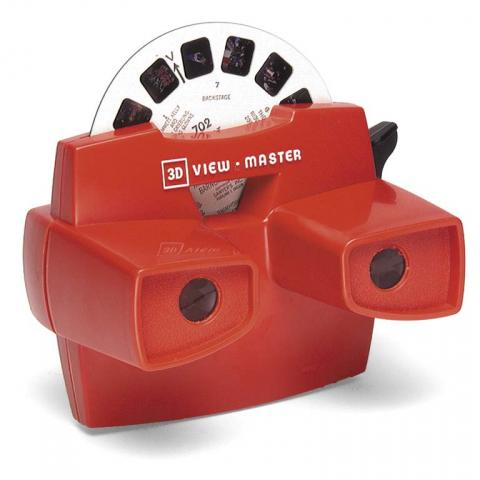
\includegraphics[scale=0.18]{viewmaster.jpg}
\captionof{figure}{Exemplaire du \it{View Master}\tss{\cite{viewmaster}}}
\end{center}


La première réalisation de la réalité virtuelle a été réalisée en 1950 avec le sensorama, un cinéma immersif crée par Morton Heilig. Il est basé sur les sensations et donne donc l'impression d'une totale immersion.
\begin{center}
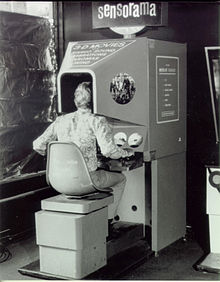
\includegraphics[scale=0.27]{sensorama.jpg}
\captionof{figure}{Modèle du sensorama\tss{\cite{sensorama}}}
\end{center}




Cette ébauche de réalité virtuelle à servit d'ailleurs pour le développement d'un simulateur de vol pour l'armée de l'air en 1966. Le premier casque de réalité virtuelle a été créé en 1970, à l'Université d'Utah par Daniel Vickers. Il est formé de 2 écrans et permet d'observer l'image virtuelle en tournant la tête.
En 1982, des  data gloves  sont créés pour permettre une sensation de réalité virtuelle encore plus importante : Ces gants se connectent à l'ordinateur et permettent d'effectuer les mouvements sur l'ordinateur.


\begin{center}
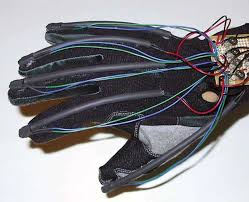
\includegraphics[scale=0.4]{data.jpeg}
\captionof{figure}{Photographie des datas gloves de 1982\tss{\cite{data}}}
\end{center}

En 1989 la société VR qui est à l'origine de l'audio sphère, des data gloves autorise Mattel, une entreprise de jeu de société à modifier les data gloves pour pouvoir l'intégrer à un jeu. Les Power gloves sont commercialisés mais ils sont assez chers et donc peu populaires.
Avec l'arrivée d'internet, la réalité virtuelle a été un peu délaissée et est restée concentrée sur le simulateur médical de vol, la conception automobile : des projets pour les professionnels.

Vers 1990, la réalité virtuelle contamine enfin les jeux vidéos avec la création du SEGA VR, par ma marque SEGA. Il est destiné à fonctionner avec la console MEGA VR. De plus des gants exosquelettes permettent l'immersion presque totale. Mais tous ces équipements coutent jusqu'à 73 000\$ et sont donc très durs à se procurer.
\begin{center}
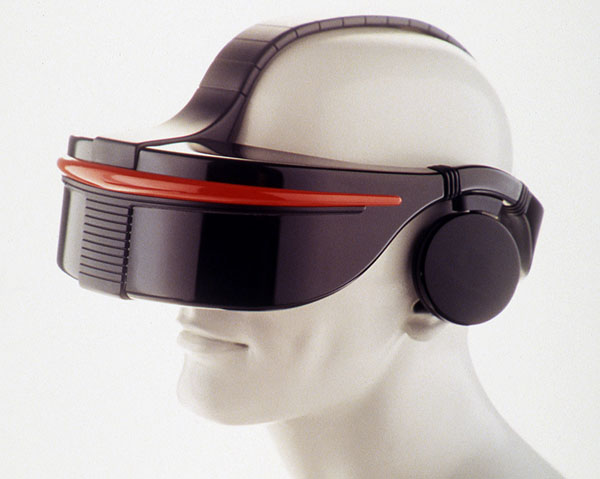
\includegraphics[scale=0.3]{sega.jpg}
\captionof{figure}{Le casque SEGA VR\tss{\cite{sega}}}
\end{center}


Nintendo, en 1990, crée le Virtual boy, un casque suivit d'une manette pour permettre une immersion totale.\\
En 2007, Google créé Google earth et Google street View, un logiciel qui permet de visualiser les habitations et les rues grâce à une vision à 360.\\
En 2014, Samsung créé son casque de réalité virtuelle le Samsung Gear VR.\\
Le 5 avril 2016, le casque HTC Vive est commercialisé.\\
Le 28 mars 2016, palmer Luckey créé l'Occulus Rift.
\begin{center}
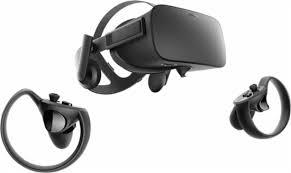
\includegraphics[scale=0.5]{occulus.jpeg}
\captionof{figure}{Le casque Occulus Rift\tss{\cite{occulus}}}
\end{center}
Mais le domaine de la réalité virtuelle est encore en plein développement !
Nous ne sommes donc qu'au début des innovations techniques sur ce sujet.

\section[Catégories de casque]{Différentes catégories de casques de réalité virtuelle}

\paragraph{Les casques VR pour smartphones}

Certains casques doivent être utilisés avec un smartphone compatible avec le casque et ce casque est généralement passif. Il compte le plus souvent un système d’accroche c’est à dire permettant la mise en place de deux lentilles qui font office de loupe. Cette méthode est plus utilisée par les consommateurs car ces casques sont beaucoup moins coûteux que les casques autonomes (prix minimal d’un casque VR pour smartphone : 100\euro{}) Il vous faut cependant un smartphone compatible et l’application pour l’utiliser  Le téléphone va donc s’occuper de toute le reste (les calculs ; le rendu, l’affichage).

Un type très particulier de casque VR pour smartphones sont les Google Cardboard. Créé par Google en 2014, ils sont fait principalement de carton (mais existent en nylon et plastique) et permettent de tester la réalité virtuelle avec un budget très serré (prix minimal : 5\,\$). Ces petits boîtiers sont donc une bonne alternative pour tester sans se ruiner. Nous en avons d’ailleurs acheté un pour pouvoir enrichir notre expérience.

\paragraph{Les casques autonomes} Il peut s'appuyer sur les capteurs de haute précision pour proposer une expérience d'immersion complète. De plus le spectateur peut aussi se déplacer librement au sein des environnements visionnés. Pour finir le casque autonome peux même retranscrire les mouvements de corps (s'accroupir ; sauter \ldots{}). Les plus connus sont l'Occulus rift et l'HTC Vive. L'Occulus Rift, bien que très médiatisé est assez peu sollicité par les professionnels car il est plutot limité. L'HTC Vive, lui, considéré comme l'excellence des casques est très populaire puisqu'il remplit toutes les charges demandées par les entreprises.

\section[Catégories de réalités]{Notion d'immersion, et différenciation des réalités}

\paragraph{L'immersion}

Lorsqu'on entend le terme de réalité virtuelle, on y associe le plus souvent le mot  immersion. En effet les caques de réalité virtuelle permettent l'immersion mais ce terme n'est pas spécifique pour ces dispositifs. \\L'immersion désigne le fait d'être complètement  plongé ou absorbé dans ou par quelque chose et ainsi pouvoir être comme  déconnecté de la réalité. Ainsi, on peut être en immersion grâce à un livre passionnant et à son histoire comme on peut l'être avec un film effrayant. Il faut donc bien prendre en compte cette notion pour éviter l'amalgame

\paragraph{Les nombreuses réalités différentes}

De nos jours, il existe de multiples catégories de réalité mais la majorité pense qu'il n'y a que la réalité virtuelle et associe donc des mauvaises définitions au terme. Celle qui se différencie le plus avec la réalité virtuelle est la réalité augmentée.\\

Rappelons le, la réalité virtuelle repose sur l'impression de réel et surtout la possibilité d'interagir avec son environnement et son corps..\\
La réalité augmentée, quant à elle, repose sur l'ajout d'objets virtuels dans un environnement réel. Elle n'obstrue pas,le plus souvent, complètement la vision du porteur de dispositif. Les caractéristiques de la réalité augmentée la rendent très attractive pour un secteur comme le tourisme. Le fait de pouvoir ajouter des informations sur l'image vue par le porteur peut par exemple servir à enrichir le déroulement de la visite d'un lieu.\\

Le port de lunettes connectées fait partie de la réalité mixe puisque l'utilisateur voit au travers de ses verres la réalité mais est superposé des objets virtuels dans le même temps.Le champ de vision est tout de même plus limité que des lunettes classiques car il faut un espace assez grand pour permettre de projeter les objets virtuels.\\

\begin{center}
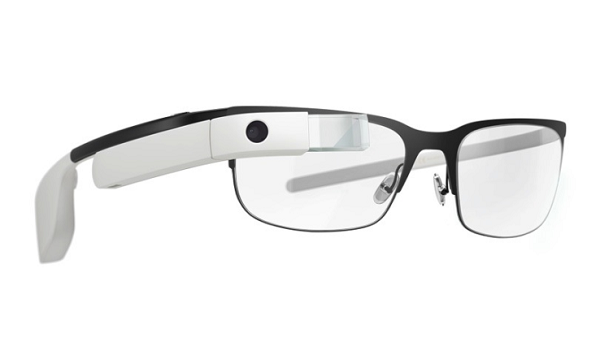
\includegraphics[scale=0.3]{glass.png}
\captionof{figure}{Photo de Google Glass\tss{\cite{formation}}}
\end{center}
On parle souvent de réalité virtuelle avec les vidéos à 360\degres{} utiles pour le tourisme pour visiter les musées à distance avec un casque, mais en réalité, elles n'appartiennent pas à la réalité virtuelle : ce ne sont que des vidéos qui sont filmées et diffusées à l'aide d'un casque de réalité virtuelle certes mais qui ne permettent aucunes interactions avec l'environnement virtuel et place l'utilisateur en tant que spectateur, ce qui est contraire au principe de réalité virtuelle.\\

On peut voir que ces nouveaux secteurs touchent de plus en plus les étudiants en informatique puisque lors de la porte ouverte de l'école Epitech, nous avons pu dialoguer avec un étudiant qui réalisait son projet sur 3 ans et qui réalisait une application utilisant la réalité augmentée : elle aura pour but d'afficher des messages virtuels sur les batiments, en ville pour que les personnes utilisant l'application puissent les apercevoir. Un autre, a réalisé un logiciel de simulation de conduite pour la réalité virtuelle.\\

Il faut donc bien différencier toutes ces catégories pour bien cerner le but de la réalité virtuelle et ses avantages malgré leurs apparences qui semblent communes.

\chapter[l'\oe il et le cerveau]{Fonctionnement de l'\oe il et impact sur le cerveau}

L'\oe il est l'organe de la vision, sens qui permet à un être vivant de capter la lumière pour ensuite l'analyser et intéragir avec son environnement.
Il peut différencier près de huit millions de nuances dans les couleurs.
Il permet donc la vue et participe à la perception de la réalité.

\begin{center}
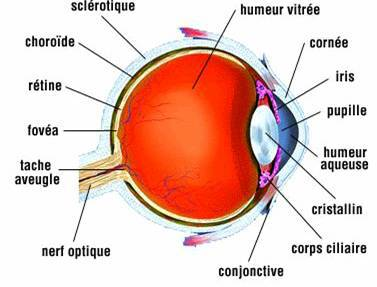
\includegraphics[scale=0.5]{oeil.jpg}
\captionof{figure}{Schéma détaillé de l'\oe il\tss{\cite{oeil}}}
\end{center}

L'\oe il est un globe orbitaire entouré par la sclérotique, un tissu fibreux et opaque qui forme le blanc de l'\oe il et qui protège l'\oe il des agressions extérieures tout en assurant le maintien de sa forme et de la cornée, une membrane transparente bombée qui réfléchit ou réfracte la lumière et qui est située juste devant l'iris.

L'humeur vitrée est un liquide transparent gélatineux qui remplit l'intérieur de l'\oe il et en assure la forme.\\
L'humeur aqueuse, produite par le corps ciliaire se trouve entre l'iris et la cornée doit nourrir la cornée et protéger le cristallin. Il est renouvelé toutes les 4 heures.

L'iris est une membrane colorée qui se situe derrière la cornée et qui, à l'aide de muscles sphincters, peut faire varier son diamètre pour réguler la quantité de lumière qui entre dans l'\oe il.

\newpage

Le cristallin est un organe particulier : il est dépourvu de tissu conjonctif, de cellules nerveuses et de capillaires sanguins. Le cristallin est composé de milliers de cellules allongés comme des rubans incurvés. Au centre du cristallin, les cellules sont parfaitement transparentes et la lumière peut donc passer.

Il est suspendu par des ligaments reliés au muscles ciliaires. Lorsque ces derniers se contractent, cela provoque un glissement des cellules du cristallin pour que le cristallin prenne une forme plus bombée. C'est l'accommodation qui consiste a augmenter la vergence du cristallin pour voir nettement les objets proches.

On peut ainsi assimiler le fonctionnement de l'\oe il à celui d'un appareil photo :
{\small}
\begin{center}
\begin{tabular}{|c|c|c|}
\hline Fonction de chaque composant & \'{E}léments de l'\oe il humain & \'{E}lément de l'appareil photo\\\hline
Régulation de la quantité de lumière& Iris & Diaphragme \\\hline
Formation de l'image & Cristallin & Lentille convergente \\\hline
Réception de l'image & Rétine & Capteur \\\hline
\end{tabular}
\captionof{figure}{Comparaison du fonctionnement de l'\oe il humain et de l'appareil photo\tss{\cite{photo}}}
\end{center}
{\small}

\begin{center}
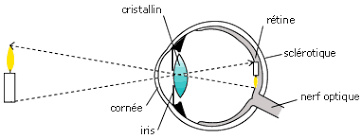
\includegraphics[scale=0.8]{schema_oeil.png}
\captionof{figure}{Schéma de la formation de l'image au niveau de l'\oe il\tss{\cite{formation}}}
\end{center}

\begin{center}
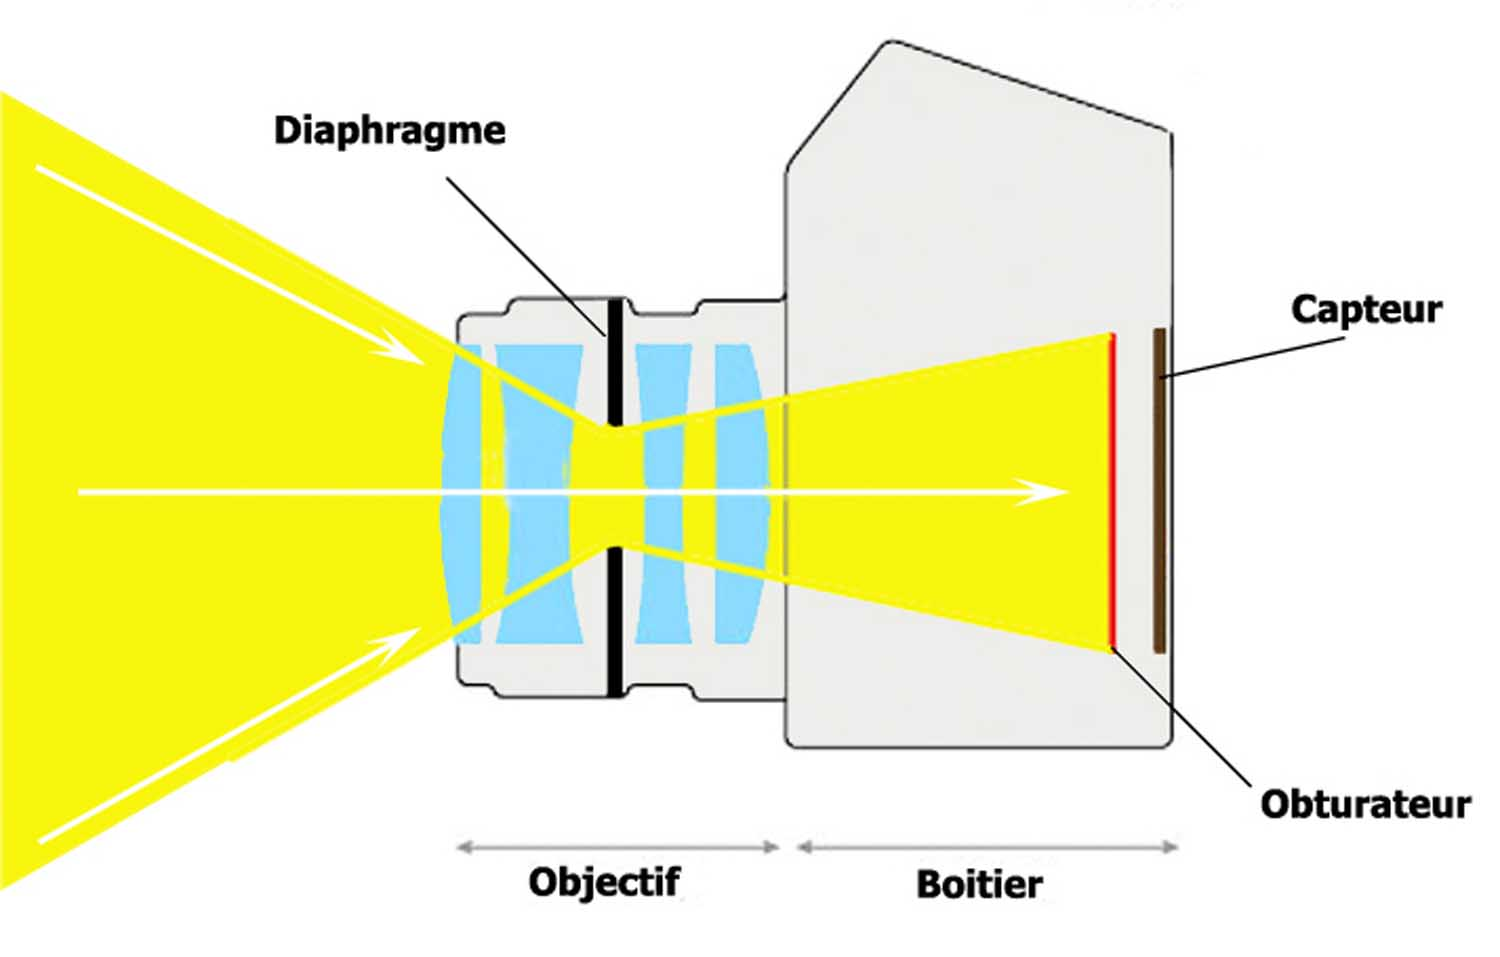
\includegraphics[scale=0.16]{appareil.jpg}
\captionof{figure}{Schéma de l'appareil photo simplifié \tss{\cite{photo}}}
\end{center}

On peut ainsi voir que les deux éléments, bien que très différents en apparence, se basent sur le même principe. L'image formée (voir schéma si dessus) se trouve sur la rétine : la rétine est une fine membrane de 0,5\,mm d'épaisseur transparente mais aussi incolore qui tapisse l'intérieur de l'il. La région sur laquelle limage se forme se nomme la fovéa, et se troue sur la macula (région où sont concentrés les cônes). La fovéa mesure 1,5\,mm de diamètre.

On peut constater que la rétine a une architecture complexe :


\begin{center}
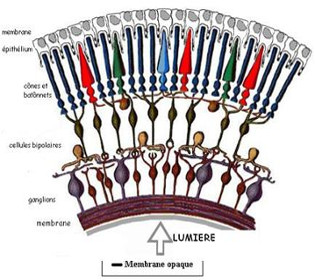
\includegraphics[]{retine.jpg}
\captionof{figure}{Composition de la rétine\tss{\cite{retine}}}
\end{center}









En effet on peut voir qu'elle possède de nombreuses couches : Tout d'abord, on peut voir qu'elle possède des photorécepteurs de deux types différents. Le cônes, sont responsables de notre perception des couleurs et il en existe 3 types différents : les rouges, les bleus et les verts. Ce sont ces cônes qui sont très concentrés au niveau de la fovéa. Les batonnets, se trouvent sur la rétine périphérique : Ils servent à capter la lumière lors de faibles luminosités. Ils sont 100 fois plus sensibles que les cônes.\\
Ensuite on peut voir deux couches de neurones : les neurones ganglionnaires et les neurones bipolaires. Ils ont pour role de transmettre les informations des photorécepteurs au nerf optique. Lorsque ces signaux électriques  parviennent au nerf optique, elles sont acheminées vers le cerveau.\\

\begin{center}
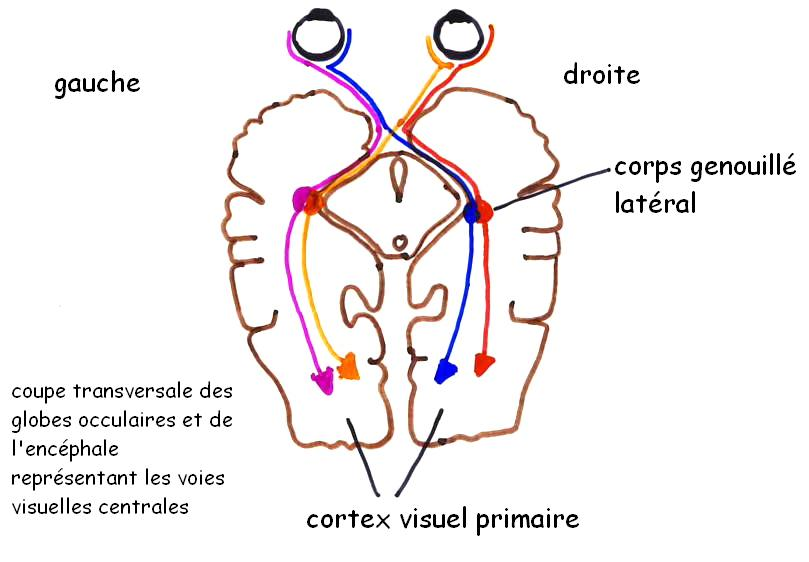
\includegraphics[scale=0.4]{cerveau.jpg}
\captionof{figure}{Schéma du cortex visuel et interaction entre cerveau et \oe il\tss{\cite{cerveau}}}
\end{center}



Ces signaux électriques sont donc acheminées vers le cerveau, plus précisément au niveau de la partie arrière du cerveau : le cortex visuel. Pour cela, le corps grenouillé latéral traite les informations de la rétine et les transmet au cortex visuel primaire.Ce dernier recoit donc les signaux électriques des yeux  et il apparait structuré comme une  carte  car chaque portion du champ de vision possède une région bien précise du cortex visuel primaire.

Cependant, le cortex visuel n'est pas la seule aire a participer pour permettre la vision. Effectivement, on a pu constater qu'il y a au moins 5 aires cérébrales qui sont utiles pour l'image. Ces aires sont responsables des formes, du mouvement\ldots{} Leur différences d'activation varient en fonction de l'image visualisée (couleurs vives, mouvements rapides\ldots{})

Le message nerveux électrique est donc traité par différentes aires cérébrales, puis le cerveau va intégrer toutes ces données et ainsi permettre la vision.

On a donc pu voir que le mécanisme de vision est très complexe mais qu'il permet de capter toutes les informations de notre environnement.

\chapter[Fontionnement]{Fonctionnement de la réalité virtuelle}

\section{Un exemple de casque autonome : L'HTC Vive}

L'HTC Vive est un casque de réalité virtuelle, né d'une collaboration entre HTC et Valve Corporation, sorti le 5 avril 2016.
La version développeur (le HTC Revive) avait des manettes avec fil, la version commerciale est sans fil.

\begin{center}
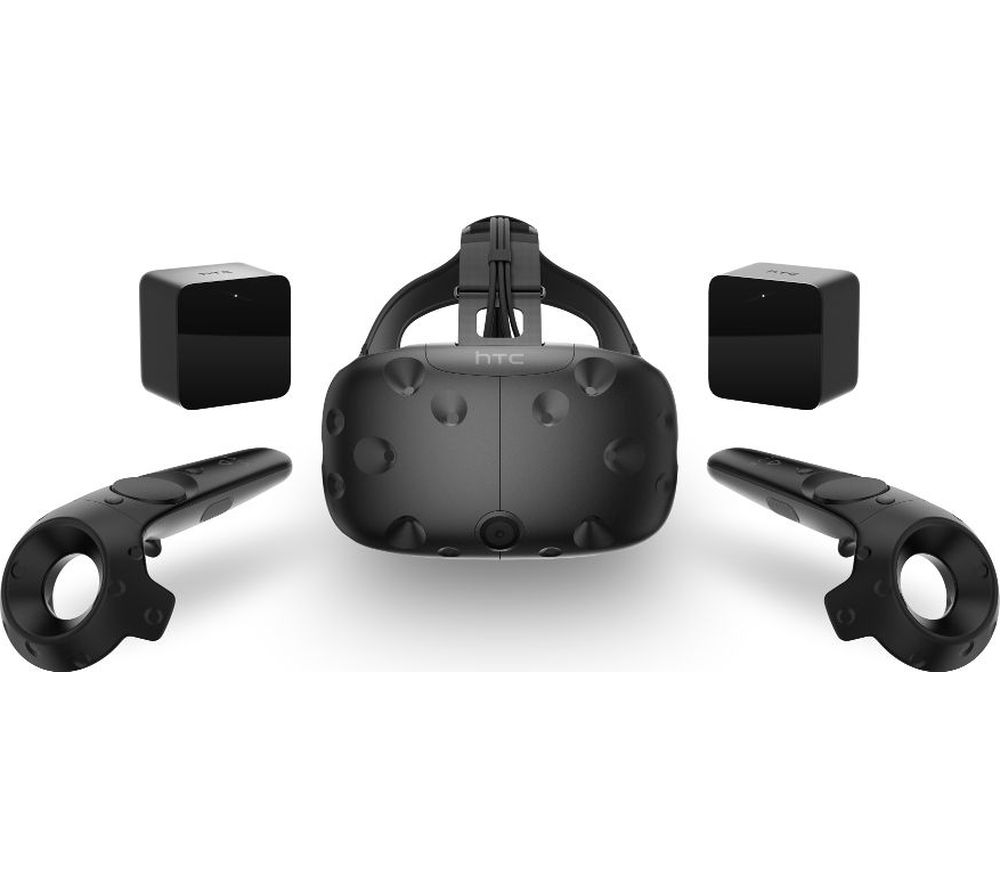
\includegraphics[scale=0.2]{htc.jpg}
\captionof{figure}{Le casque de réalité virtuelle HTC Vive\tss{\cite{htc}}}
\end{center}

\paragraph{Fiche produit :}
\begin{itemize}
\item Famille : Casque autonome
\item Environnement qui permet la bascule des écrans : Steam VR (ordinateur $\leftrightarrow$ casque)
\item Système d'exploitation nécessaire sur le PC pour utiliser le casque : Windows 7 ou plus.
\item Résolution : 2160 $\times$ 1200 pixels (1200 $\times$ 1080 pixels pour chaque \oe{}il)
\item Taux de rafraichissement : 90\,Hz
\item Connectivité : HDMI, DisplayPort, USB, Jack
\item Fonctionnalités : L'HTC Vive est composé de capteurs comme le gyroscope, l'accéléromètre et des capteurs de position laser.
L'écart pupillaire peut se régler manuellement à l'aide d'une mollette, située sur le coté droit du casque, ainsi que la distance entre les yeux et les optiques à l'aide de deux autres mollettes au niveau des attaches.
 Il comporte aussi une prise jack pour brancher des écouteurs et écouter du son en 3D ou utiliser les écouteurs fournis, ainsi qu'une prise USB pour des éventuelles extensions. Une caméra est intégrée sur la face avant, elle permet de controler l'environnement extérieur sans enlever le casque. Un micro permet quant à lui de parler dans les jeux multi-joueurs, ou de répondre à des appels téléphoniques via  Bluetooth vers un téléphone portable.
\item Prix : 700\euro{} pour la premère version et 1300\euro{} pour la version professionnelle.
\end{itemize}

\section[Fontionnement de l'HTC Vive]{fonctionnement du casque autonome}

Que ce soit l'Occulus Rift, l'HTC Vive ou l'OS Vr, ils se basent tous sur le même principe
\begin{center}
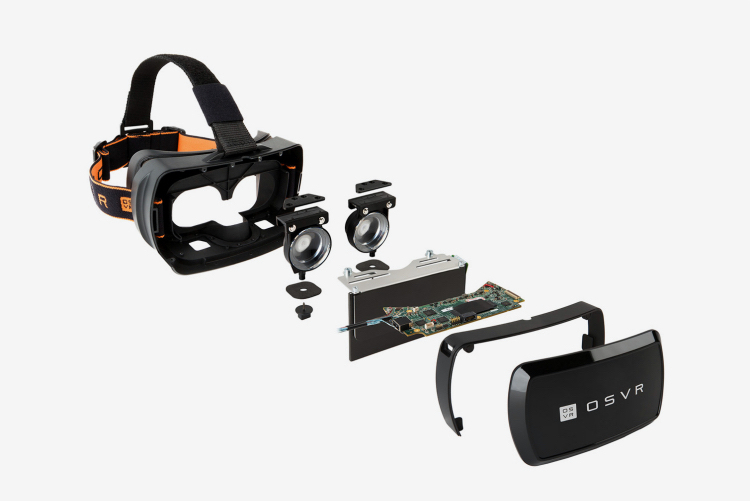
\includegraphics[scale=0.3]{eclate.jpg}
\captionof{figure}{Schéma éclaté d'un casque de réalité virtuelle\tss{\cite{eclate}}}
\end{center}

Tout d'abord, on peut voir que la structure du casque est faite pour que l'utilisateur soit en position confortable. Le maintien est assuré par les nombreuses sangles qui compensent le poids du dispositif. On peut donc parler d'ergonomie du boitier.

L'élément le plus fondamental est l'écran. Il doit être ultra haute définition. Il est bien sur intégré et est légèrement plus grand qu'un écran de smartphone. Sur l'écran, deux images sont affichées. Ces casques fonctionnent par stéréoscopie, technique grâce à laquelle le cerveau percoit un relief. Il percoit un relief en reconstituant une image à partir des deux images planes et différentes percues par chaque \oe{}il. Ces images stéréoscopiques sont crées par deux lentilles situées en face de chaque \oe{}il. Chaque image est destinée à un \oe{}il.
On constate que les deux images sont légèrement décalées.

\begin{center}
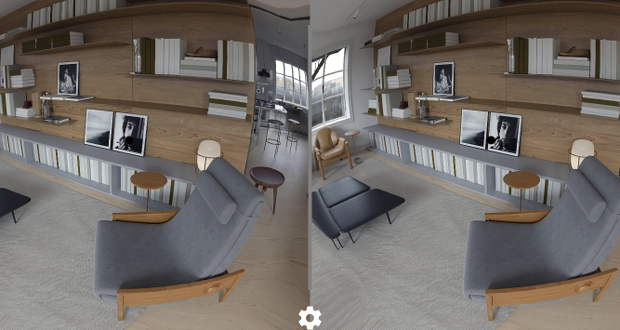
\includegraphics[scale=0.5]{ecran.jpg}
\captionof{figure}{Photographie représentant l'écran du casque\tss{\cite{ecran}}}
\end{center}

Les lentilles sont au nombre de 2 et elles sont quasiment collées aux yeux et permettent de dissocier l'image correspondant à chaque il et ainsi reproduire notre vision binoculaire. Il est nécessaire pour apprécier les distances, la profondeur, et le relief, il faut que notre cerveau recoivent des signaux électriques de nos deux yeux. C'est e même procédé qui est utilisé pour les manettes de jeux : elles comprennent 2 ou 3 caméras pour avoir une très grande précision.
 Le champ de vision doit aussi être reproduit : l'angle de vision du casque est de 90\degres{} latéralement et de 110\degres{} en diagonale, ce qui est très proche de la réalité (vie réelle : 120\degres{}).

 Pour permettre une meilleure immersion, des écouteurs sont intégrés au casque.
Des leds infrarouges, situées sur les lunettes et le bandeau arrière permettent de détecter les mouvements de l'utilisateur. Une mini caméra placé à coté de l'utilisateur localise le casque dans une zone de 9\,m\tss{2}.

Le logiciel Reality Adjacent Tracker, intégré à une carte mère assure le suivi des mouvements de la tête. Il combine trois technologies : l'accéléromètre pour mesurer les déplacements latéraux, le gyromètre qui est utilisé pour les mouvements de rotation et le magnétomètre qui agit comme une boussole.

Enfin, le délai entre le mouvement réel et sa retranscription à l'écran doit être très rapide pour vraiment donner l'impression de réel : pour l'Occulus rift, ce temps est de 25 millisecondes et pour l'HTC Vive, il est de 10 millisecondes environ. Ce temps de latence, s'il est trop long, peut provoquer la nausée.

\section[\'{E}tude statistique]{\'{E}tude sur la popularité de la réalité virtuelle}

Pour connaitre la renommée de la réalité virtuelle, nous avons décidé de réaliser un sondage au niveau du lycée sur le sujet de la réalité virtuelle avec 8 questions, grâce au logiciel Survio. Nous l'avons envoyé à tous les élèves du lycée soit 1545 élèves. Nous avons recueillis à ce stade 547 réponses ce qui représente plus d'un tiers des élèves. Le logiciel ne permet que d'étudier 203 réponses sur les 547, dont voici les résultats :


\begin{center}
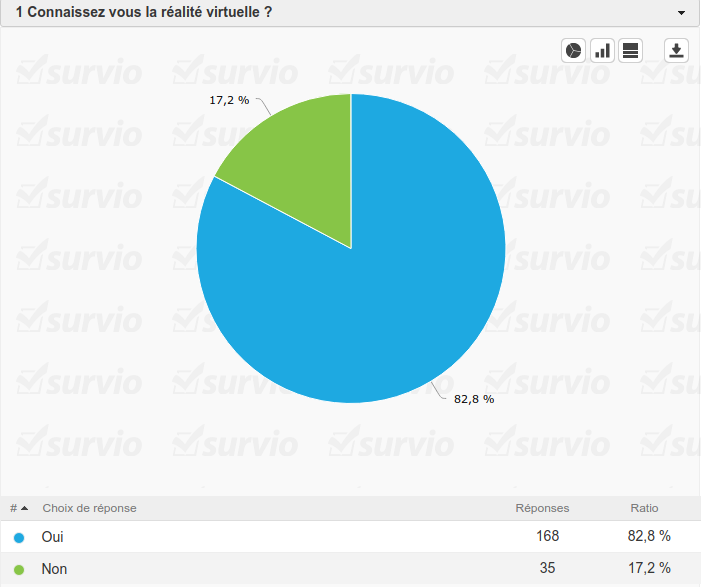
\includegraphics[scale=0.5]{1.png}
\captionof{figure}{Diagramme circulaire pour la question n\degres{}1\tss{\cite{etude}}}

Ici on peut remarquer que le sujet de la réalité virtuelle n'est pas inconnu pour la plupart des jeunes mais une petite partie n'en a tout de même jamais entendu parler
\end{center}

\begin{center}
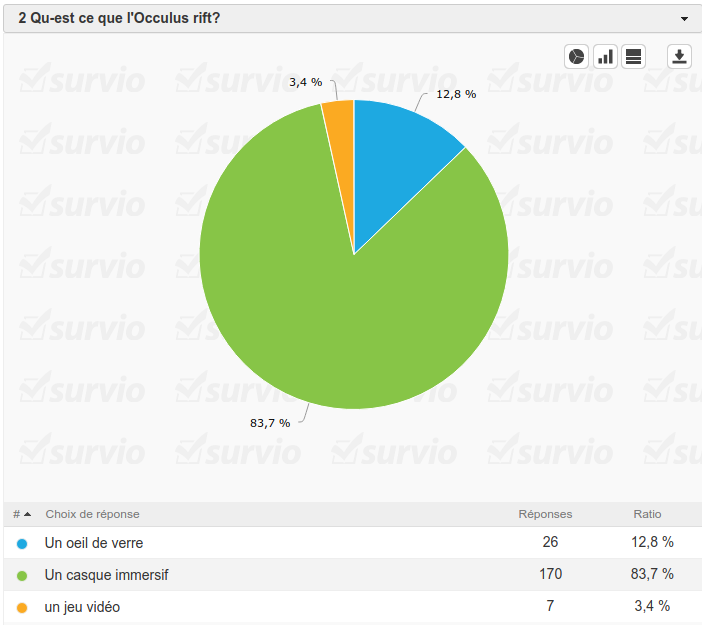
\includegraphics[scale=0.5]{2.png}

La plupart des jeunes savent ce qu'est un Occulus Rift mais 16,5\,\% de ces derniers se sont trompés.
\end{center}

\begin{center}
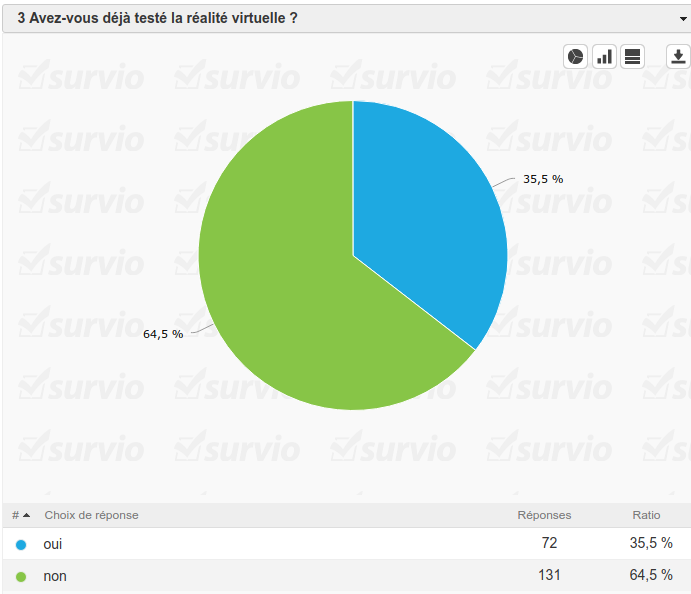
\includegraphics[scale=0.5]{3.png}

Ici on voit que la réalité virtuelle est assez accessible pour l'essai puisque 65\,\% des jeunes ont déja testés.
\end{center}

\begin{center}
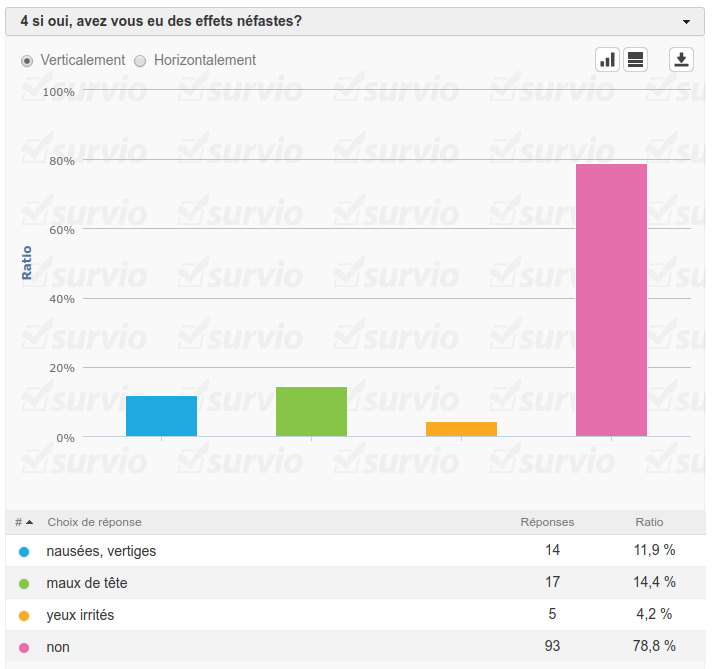
\includegraphics[scale=0.5]{4.png}

 On observe que la majorité des jeunes n'a pas eu d'effets néfastes suite à l'utilisation de la réalité virtuelle mais une partie non négigeable a tout de même ressentis quelques symptômes
\end{center}

\begin{center}
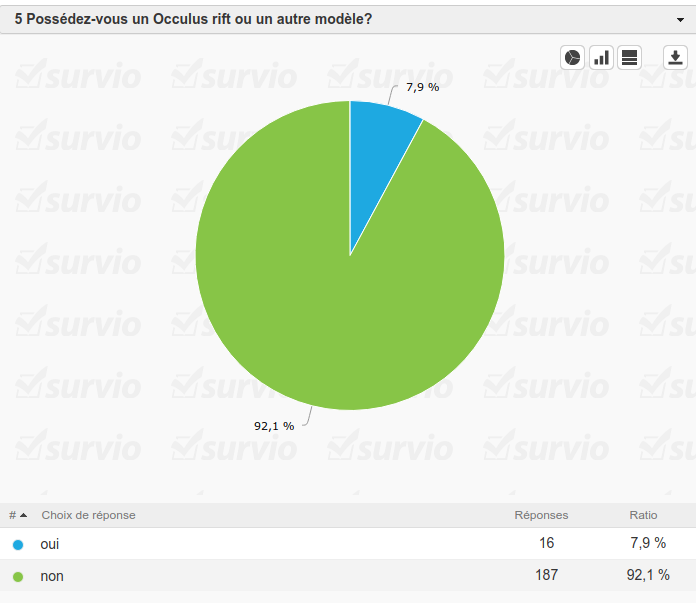
\includegraphics[scale=0.5]{5.png}

Les casques de réalité virtuelle sont très chers ce qui explique que très peu de personnes en possède un.
\end{center}

\begin{center}
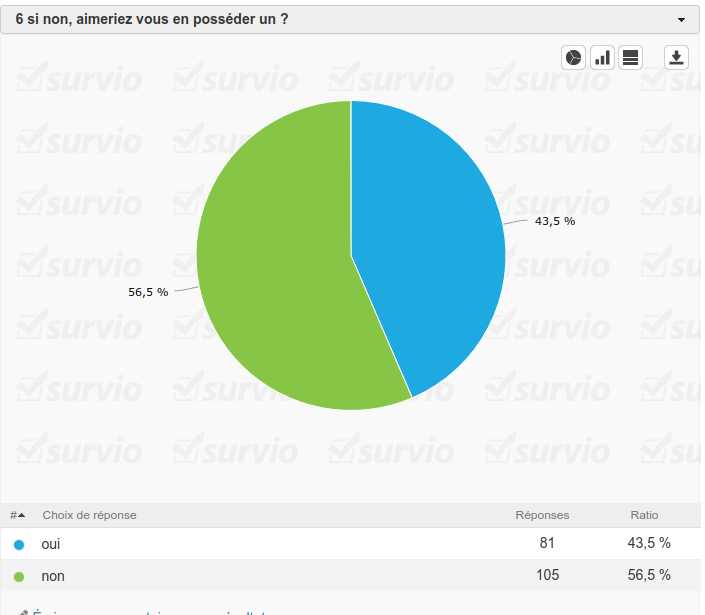
\includegraphics[scale=0.5]{6.png}

Uniquement certaines personnes en veulent un.
\end{center}

\begin{center}
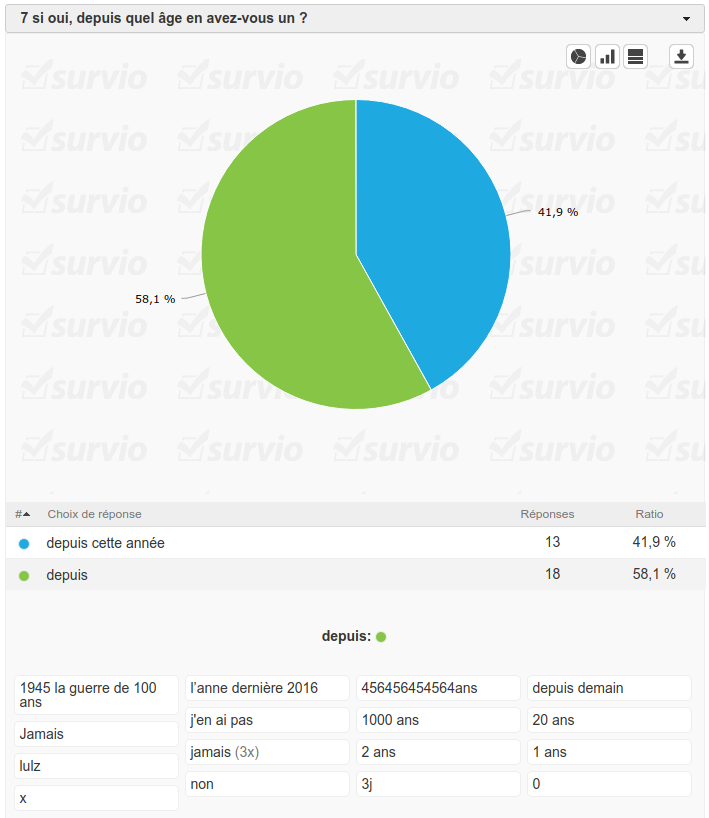
\includegraphics[scale=0.4]{7.png}

On voit ci que certains resultats sont à négliger mais on voit tout de même que ce qui en possèdent ne l'ont pas depuis longtemps
\end{center}

\begin{center}
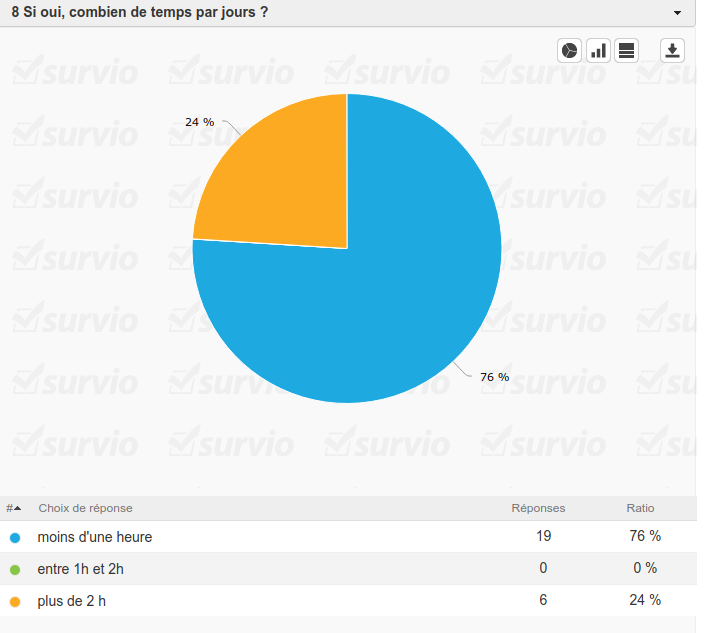
\includegraphics[scale=0.5]{8.png}

On peu voir que les jeunes sont sérieux pour la majorité et qu'il ne l'utilise pas dans l'excès
\end{center}

\newpage

\section[\'{E}xpérience et sensations]{Expérience avec la VR et sensations éprouvées}

Nous voulions, pour enrichir notre TPE et avoir notre propre expérience, tester la réalité virtuelle et avoir l'avis d'un professionnel sur le sujet. Après de nombreuses recherches sur les différentes entreprises, nous avons choisi de contacter l'école d'informatique  Epitech à Nancy et l'entreprise Human Games.

L'école Epitech est une école d'informatique et de code localisée dans plusieurs grandes villes y compris Nancy. On y effectue un cursus en 5 ans et on développe tout au long des années de grandes capacités de code et d'informatique. Nous y sommes allés lors des portes ouvertes et nous avons pu visiter l'établissement ainsi que poser quelques questions sur la réalité virtuelle. Nous avons également pu recueillir des témoignages de jeunes qui avait réalisé des logiciels pour différentes réalités. Grâce à cela, nous avons déjà pu enrichir notre dossier. Nous avons ensuite décidé de rencontrer une entreprise pour avoir d'autres conseils et pouvoir tester un casque de réalité virtuelle.


Nous avons donc contacté l'entreprise Human Games. Nous nous y sommes rendus pendant les vacances de Noël et nous avons pu recueillir de très nombreux conseils sur les différentes catégories de réalité et sur les différents casques. Ensuite, nous avons eu la chance de tester l'HTC Vive. L'HTC Vive fonctionne avec des capteurs et des manettes.

\begin{center}
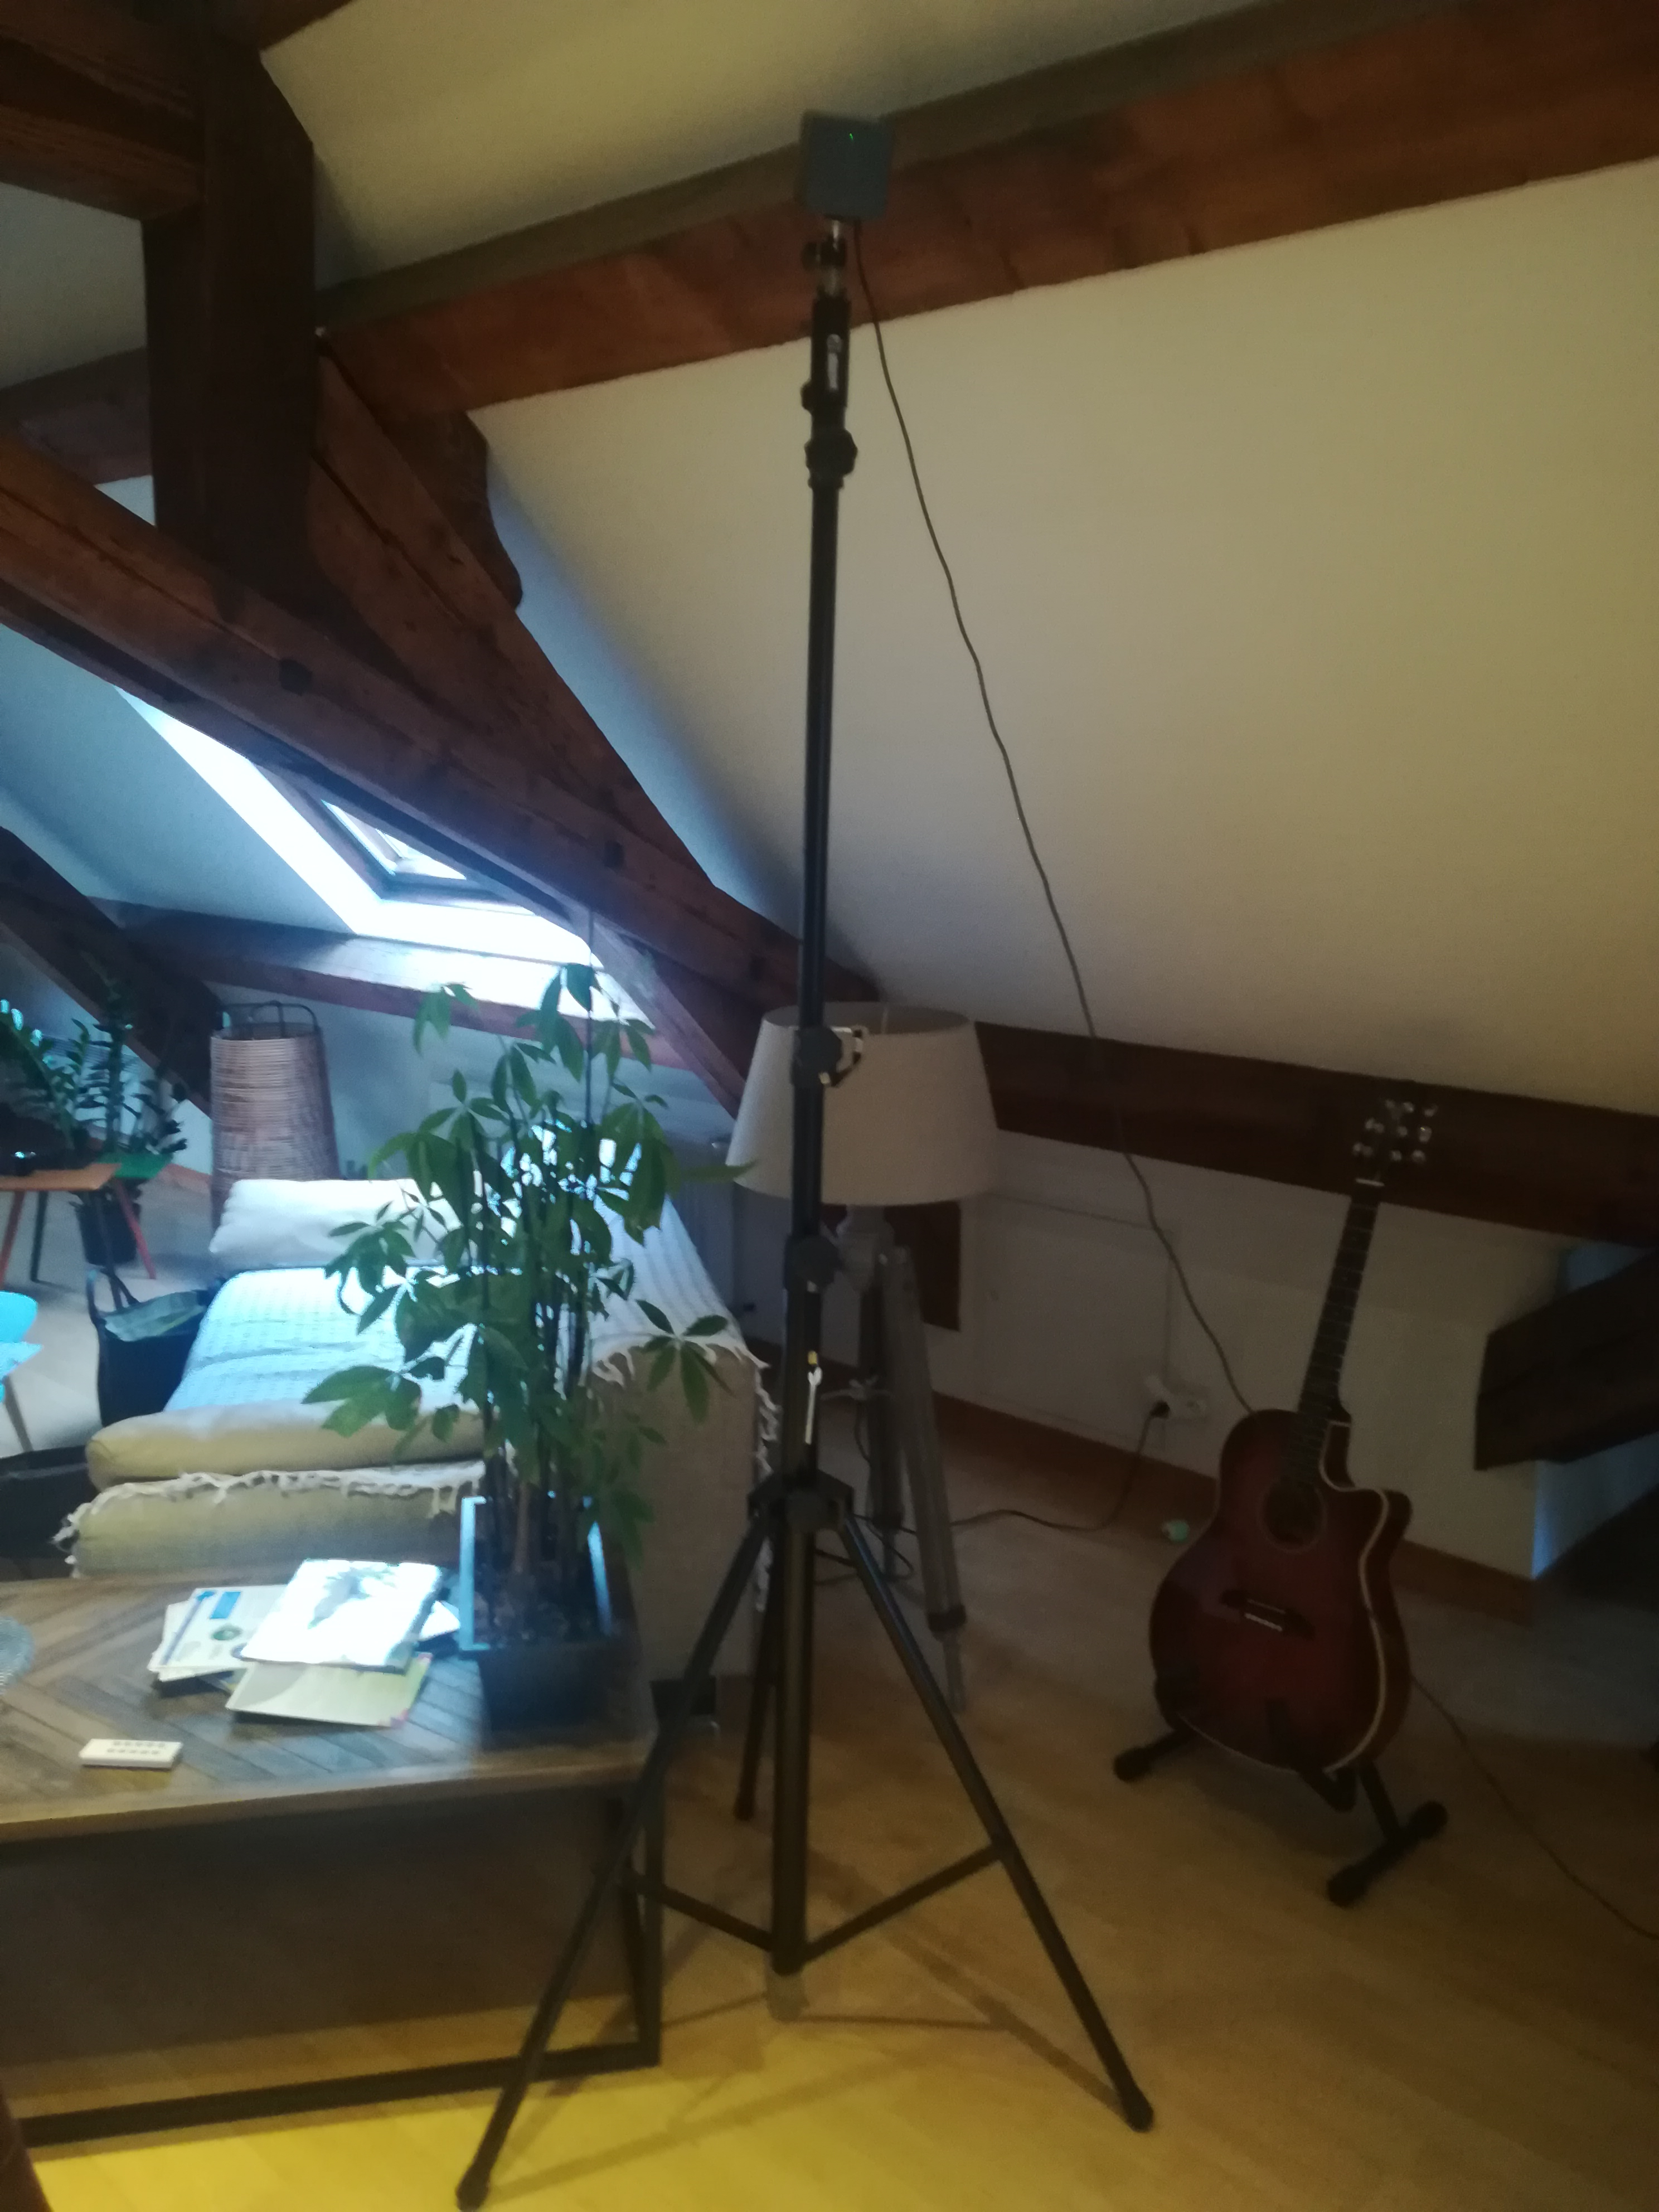
\includegraphics[scale=0.04 ]{capteur.jpg}
\captionof{figure}{Photographie d'un capteur nécessaire pour le fonctionnement du casque}
\end{center}


\begin{center}
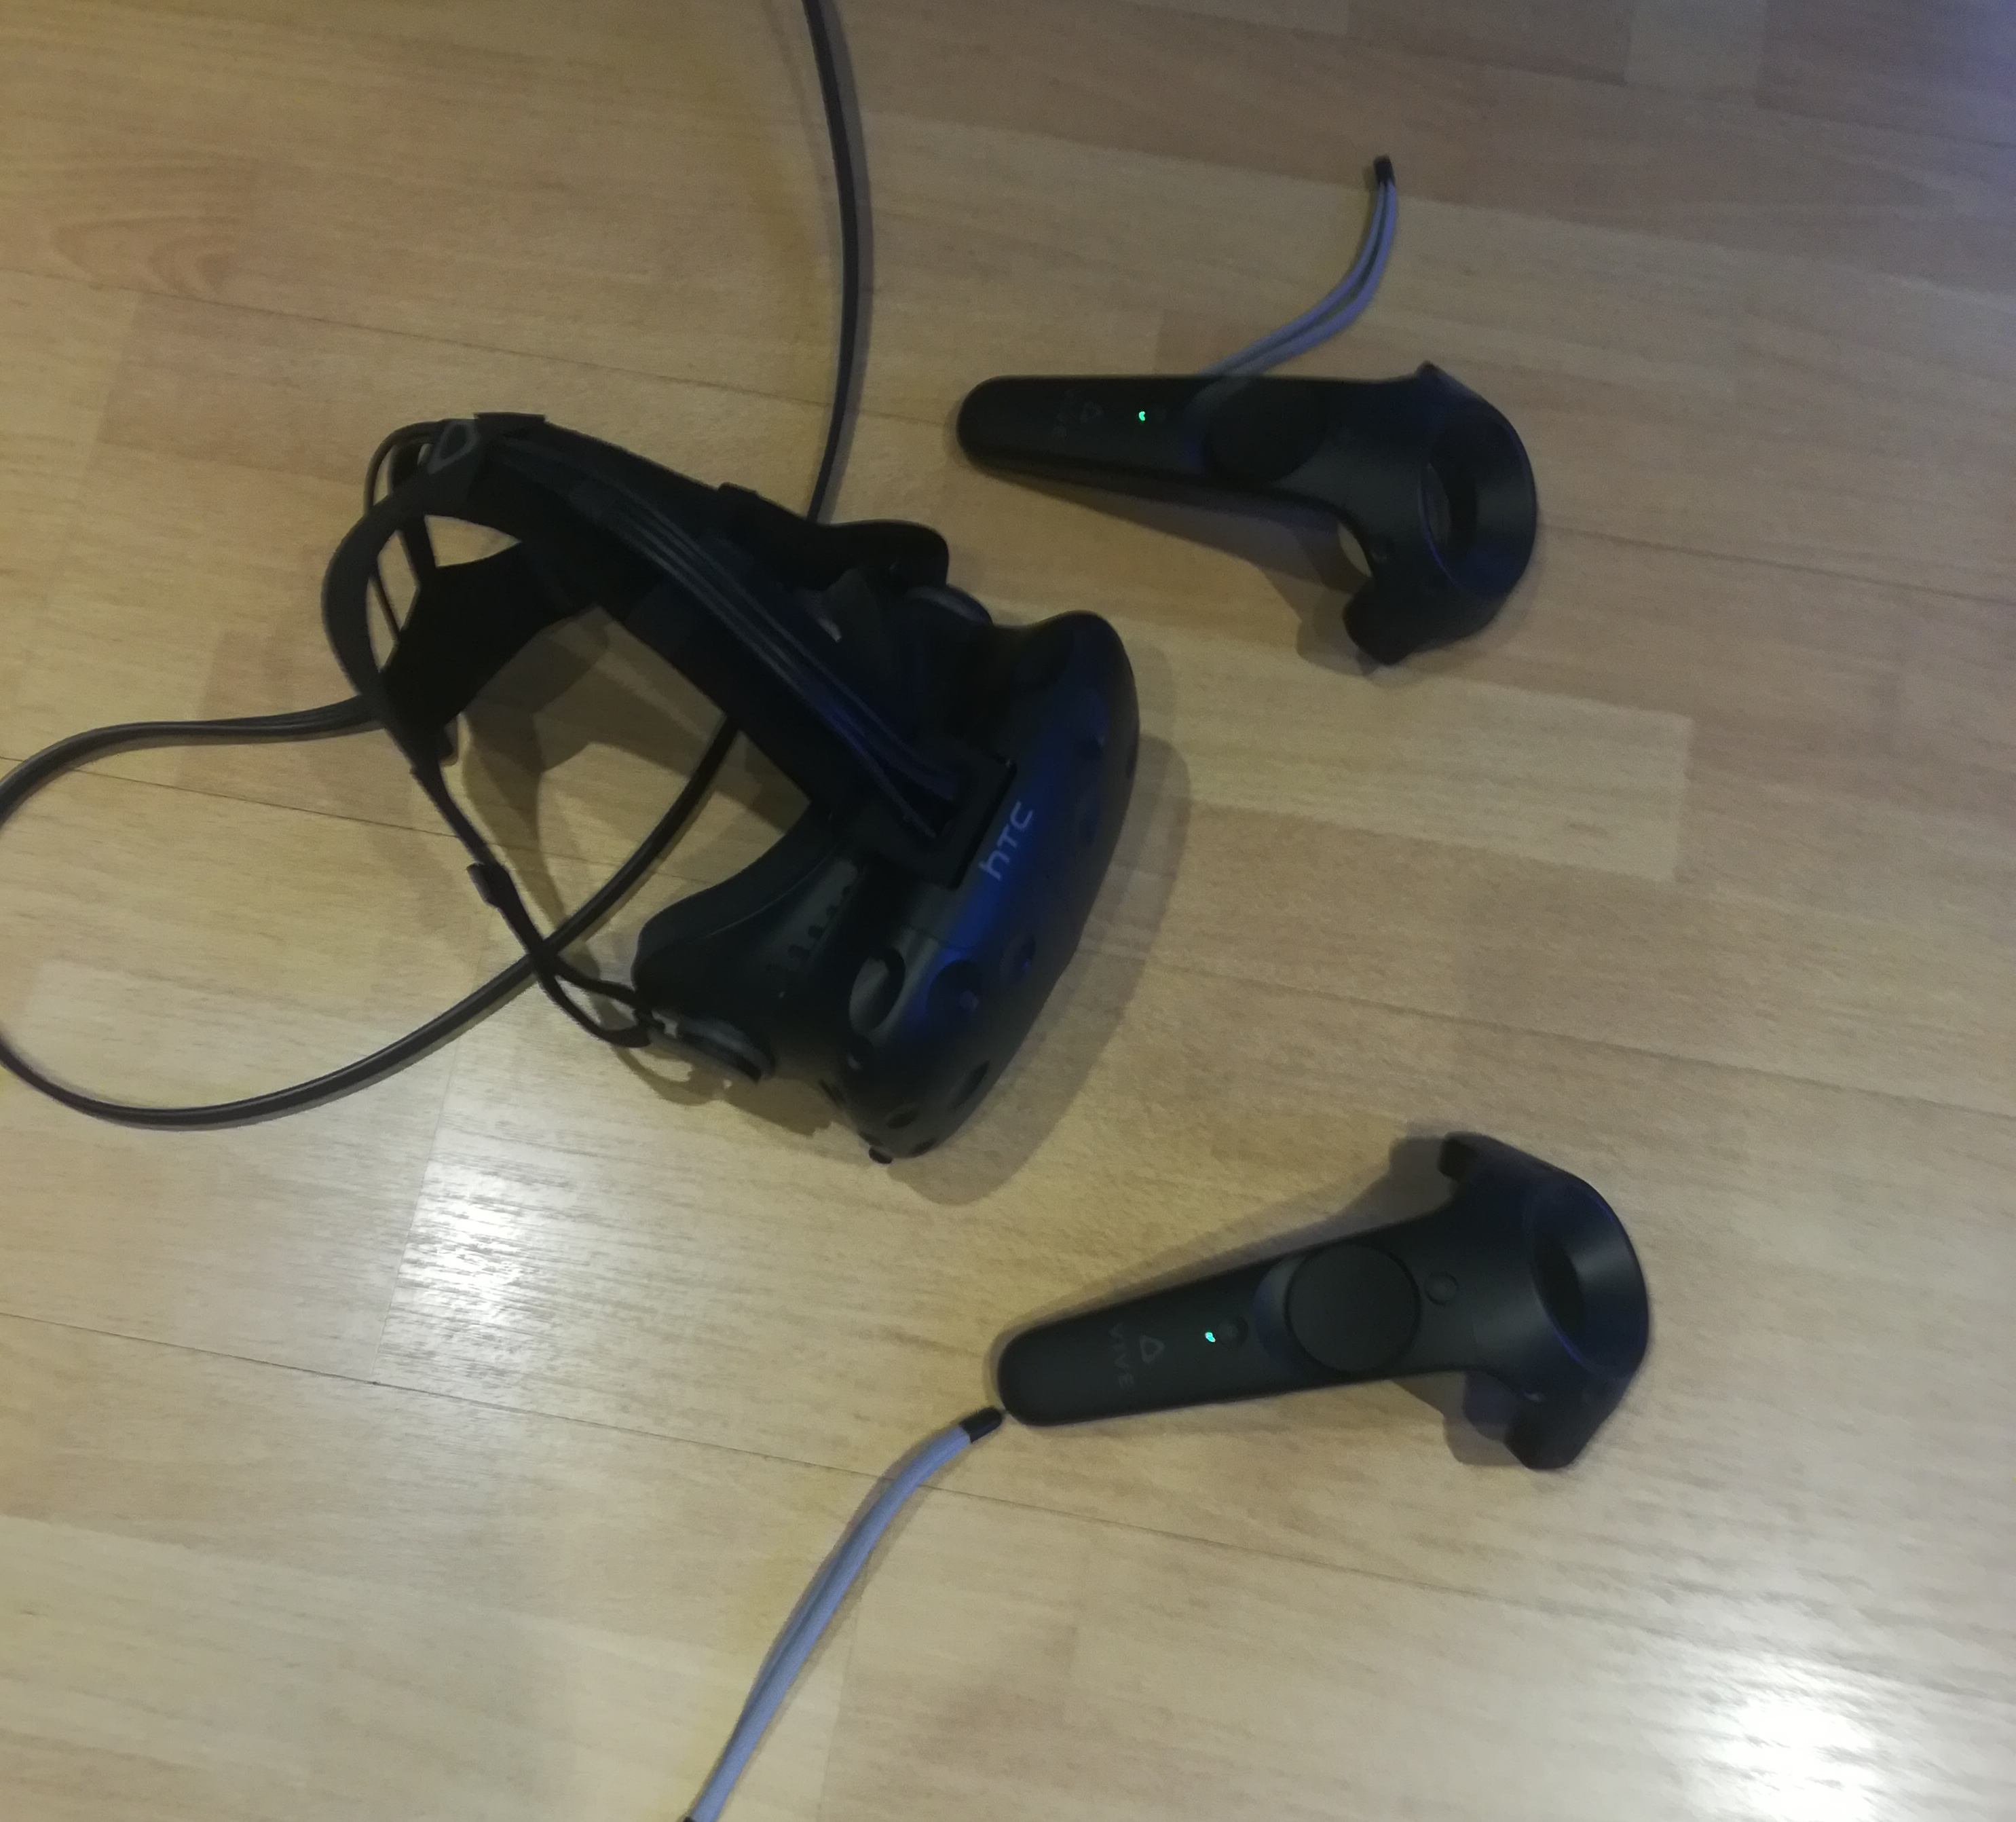
\includegraphics[scale=0.05]{casque.jpg}
\captionof{figure}{Photographie du dispositif}
\end{center}


\begin{center}
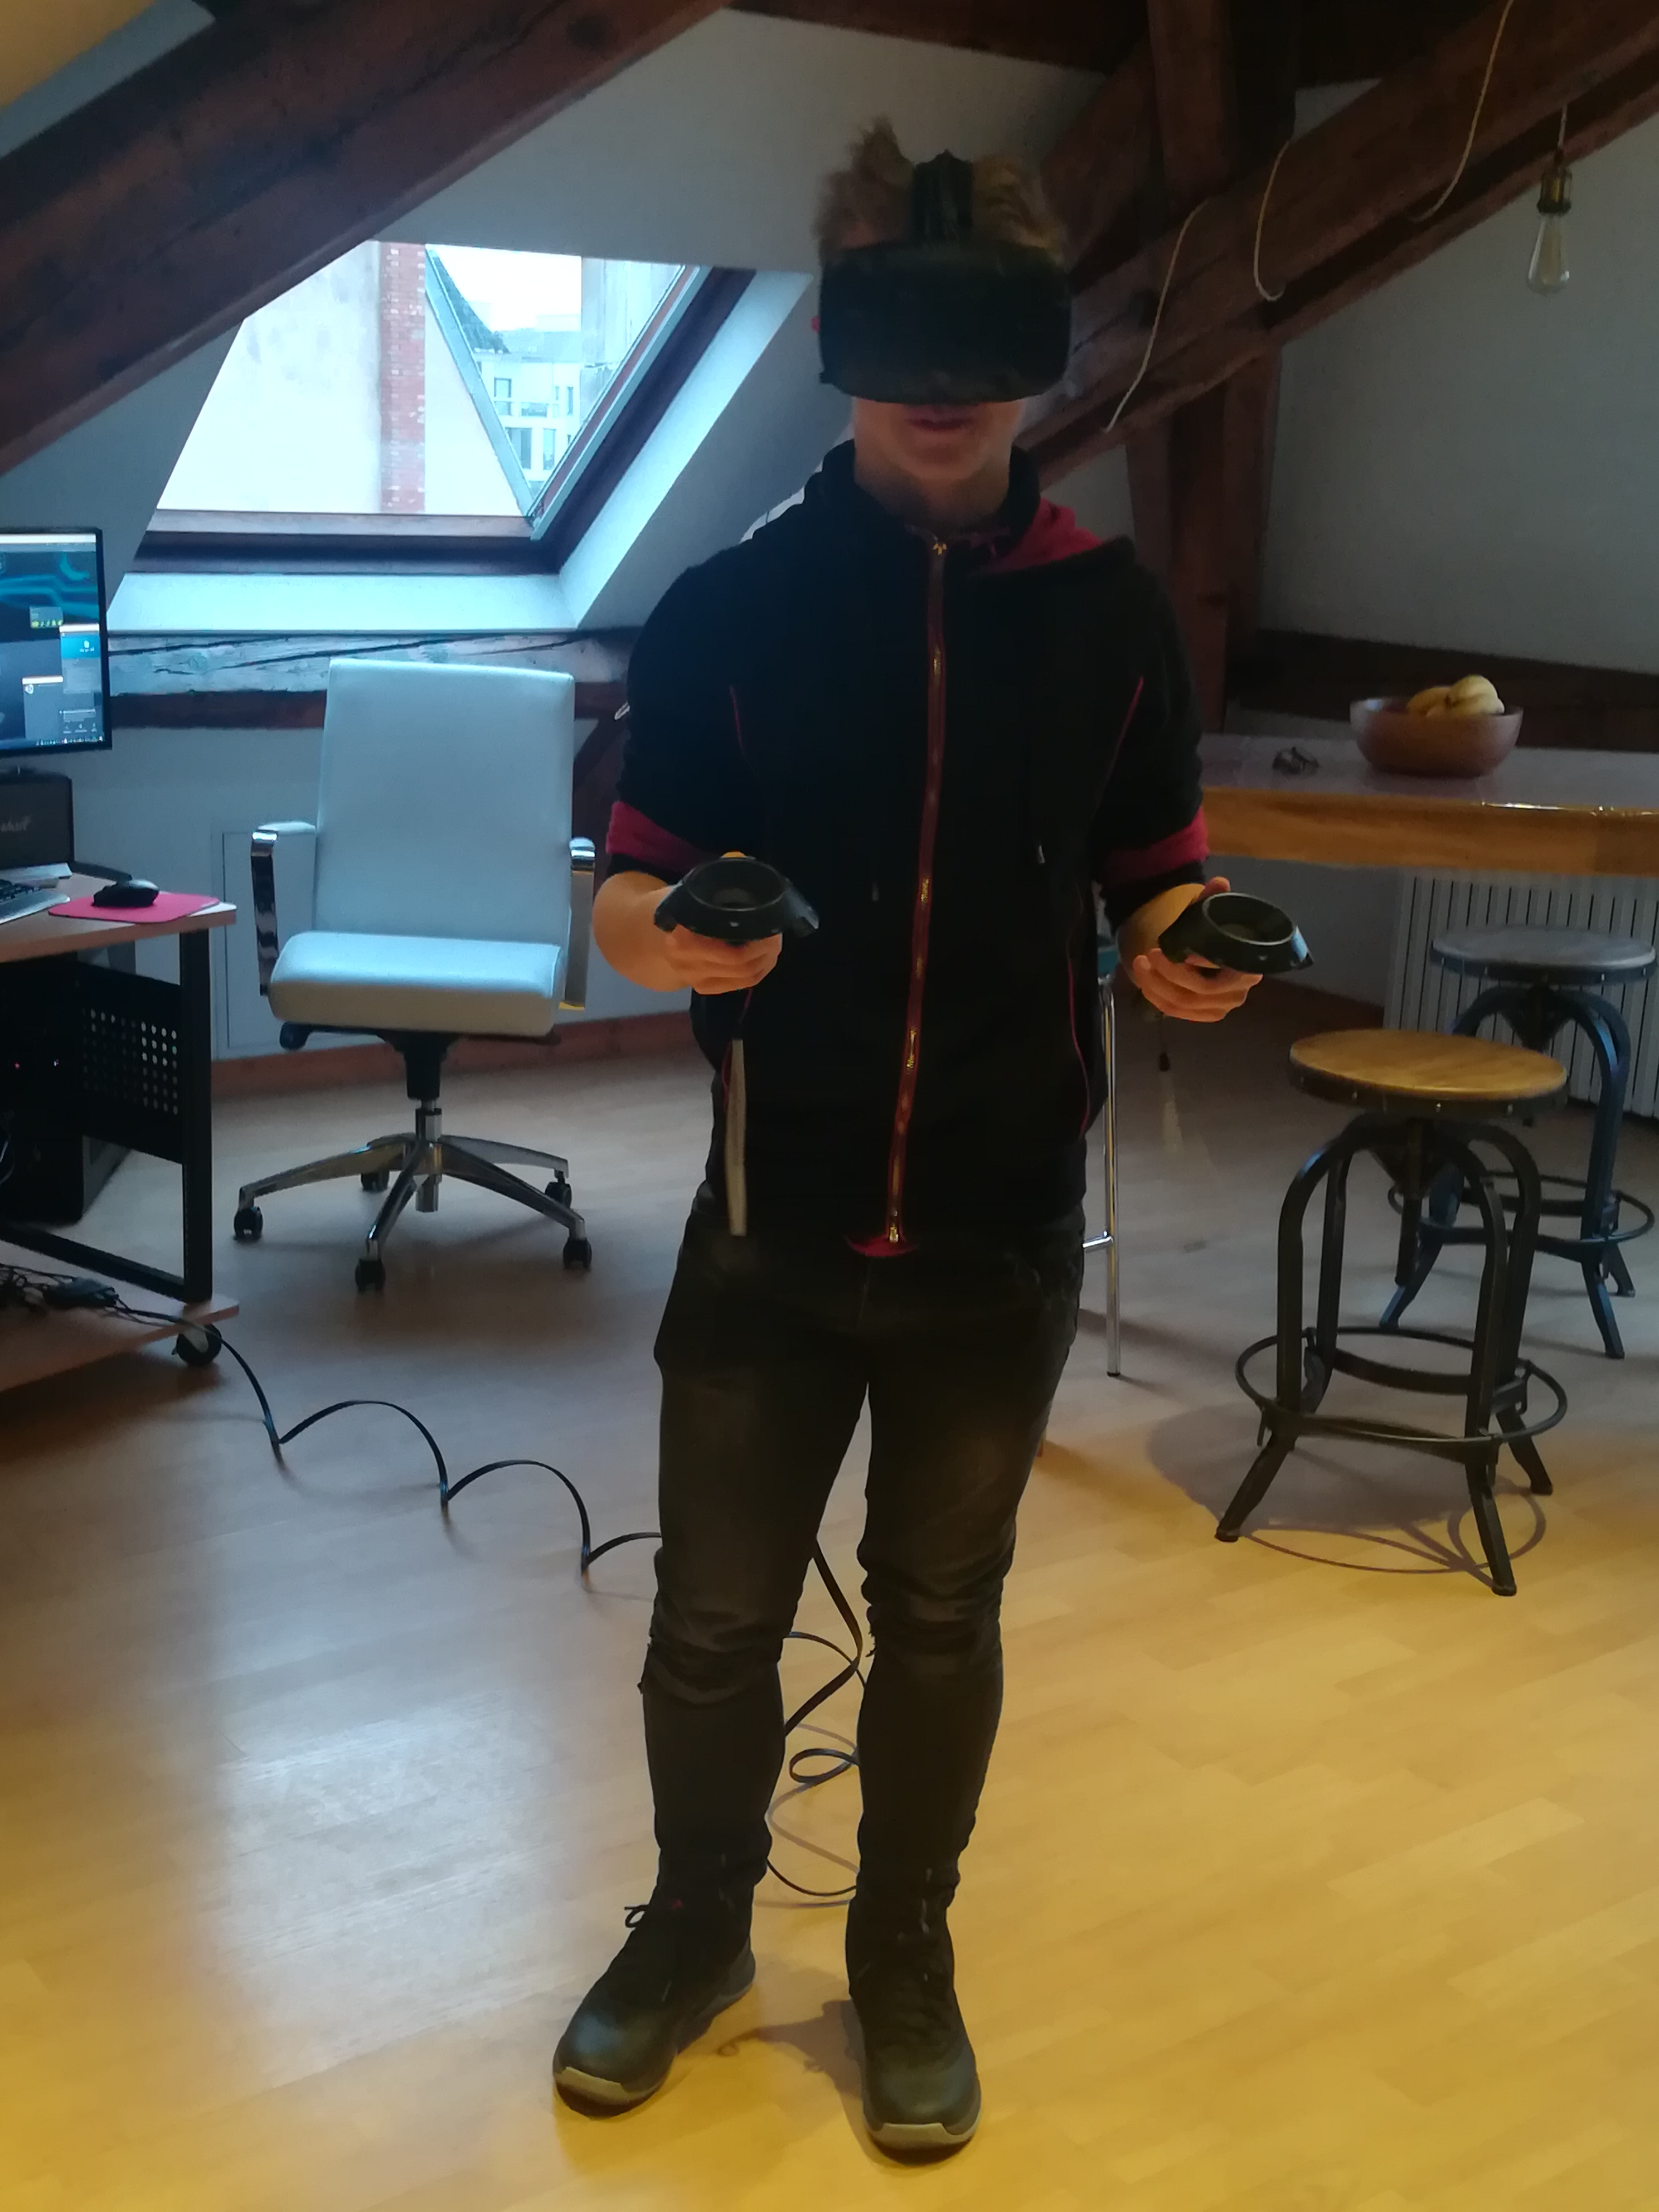
\includegraphics[scale=0.04]{nicolas.jpg}
\captionof{figure}{Nicolas prêt à utiliser le casque et les manettes}
\end{center}

 Nous avons pu évoluer dans un environnement composé de nombreuses activités comme prendre un objet, mixer, ou encore éclater des ballons. Ensuite, nous avons réalisé un test sur le gaspillage de l'eau où l' on évoluait dans une maison et l'on effectuait les taches quotidiennes. Nous avons aussi testé un simulateur de rue et on a même pu se faire renverser par une voiture de facon virtuelle ! Les sensations étaient au rendez-vous ! L'immersion étaient totale et nous avons vraiment apprécié ce moment.



 Durant l'expérience, aucune personnes du groupe n'a subi d'effets néfastes mais lors de la fin de l'expérience, lorsqu'on retire le casque, nous avons eu des légers vertiges et nous avons eu besoin d'une minute pour nous resituer dans la pièce. Nous sommes très chanceux d'avoir pu tester un casque de réalité virtuelle et cette expérience aura été très enrichissante pour notre culture personnelle et pour rapport.


 \part[Innovations et dangers]{Les innovations par l'immersion et les dangers pour la santé}

 \chapter[Innovations]{Innovations et changements radicaux par l'immersion}

 \section{Fonction ludique}

Dans le domaine du jeu vidéo, la réalité virtuelle ne se développe pas encore énormément ; c'est-à-dire que les gamers voudraient des jeux programmés et créés spécialement pour la réalité virtuelle, or il n'existe pour le moment que des adaptations de jeux vidéo, c'est-à-dire un jeu qui était de base en 2D qui a été adapté pour la 3D, comme résident evil, skyrim ou encore Until dawn. Cependant l'effet d'immersion reste présent et très appréciable, notamment il est possible d'interagir avec son environnement et d'être réellement à la place du personnage que l'on jouait devant l'écran avant. Il faut cependant prévoir le budget, puisqu'il est nécessaire de posséder un ordinateur puissant et une carte vidéo de très bonne qualité pour gérer la quantité phénoménale d'informations (ordinateur avoisinant les 800-1200\euro) ainsi qu'un casque de réalité virtuelle (550-820 \euro en fonction du casque) Cependant la sortie récente du PlayStation VR (400 \euro et fonctionnant avec la PlayStation) permettra peut-être de faire baisser le prix des casques et d'augmenter le développement des jeux spécialement pour la réalité virtuelle.

\vspace{0.5cm}

\noindent Configuration minimale requise chez Nvidia :
\begin{itemize}

\item GPU : Carte graphique NVIDIA GeForce GTX 1060 ou plus
\item CPU : Processeur Intel Core i5-4590 ou plus
\item Mémoire système : 8 Go de RAM ou plus
\item Sortie vidéo : HDMI 1.3 (x1)
\item Connectique : USB 3.0 (x3)
\item Système d'exploitation : Windows 7 Service Pack 1 (64 bits) ou plus
\item Pilote : GeForce 359 ou plus

\end{itemize}


\section[Avantages]{Les progrès et les avantages de cette technologie}

La réalité virtuelle est en plein développement et mène un véritable révolution dans notre société. Cette technologie est diffusé dans plusieurs domaine comme la médecine, le sport, la science ; elle va améliorer notre quotidien dans les années à venir.
Voici quelques apercus de cette nouvelle technologie :
\begin{itemize}
  \item Vivre sur Mars : la NASA prévoit d'utiliser la réalité virtuelle afin de simuler et expérimenter la vie sur la planète rouge : cette technologie (simulation) entraine efficacement les astronautes à l'environnement qu'ils devront affronter lors de leur mission.

  \item Apprendre à opérer : le monde de la chirurgie requiert de nombre savoirs et de l'expérience : c'est donc une discipline complexe, qui demande de nombreuses heures d'apprentissage. La venu de la réalité virtuelle dans ce milieu médical pourrait être une véritable révolution. Pour quelques étudiants en médecine chanceux, ils vont pouvoir réaliser une opération virtuelle pour ainsi être mieux préparés et éviter de faire des erreurs au niveau débutant.

  \item Calmer la douleur : Pour les brulés, le docteur Hoffman a mené une expérience pendant leur séance de nettoyage quotidienne qui ouvre leurs plaies de nouveau. Il a fait appel à la réalité virtuelle pour éviter d'avoir recours à la morphine ou autres substances ayant le même objectif. En effet, il suffit d'immerger un brulé dans des terres gelées, loin du feu, de la douleur et de l'eau qui coule sur leurs blessures. Les résultats ont été sans appel, la partie du cerveau réservée à la douleur est bien moins activé naturellement.

  L'endorphine est une hormone produite par le complexe hypothalamo-hypophysaire. L'hypothalamus produit des hormones qui remplissent un bon nombre de fonctions corporelles. L'hypophyse elle, régule les hormones.
\end{itemize}

\begin{center}
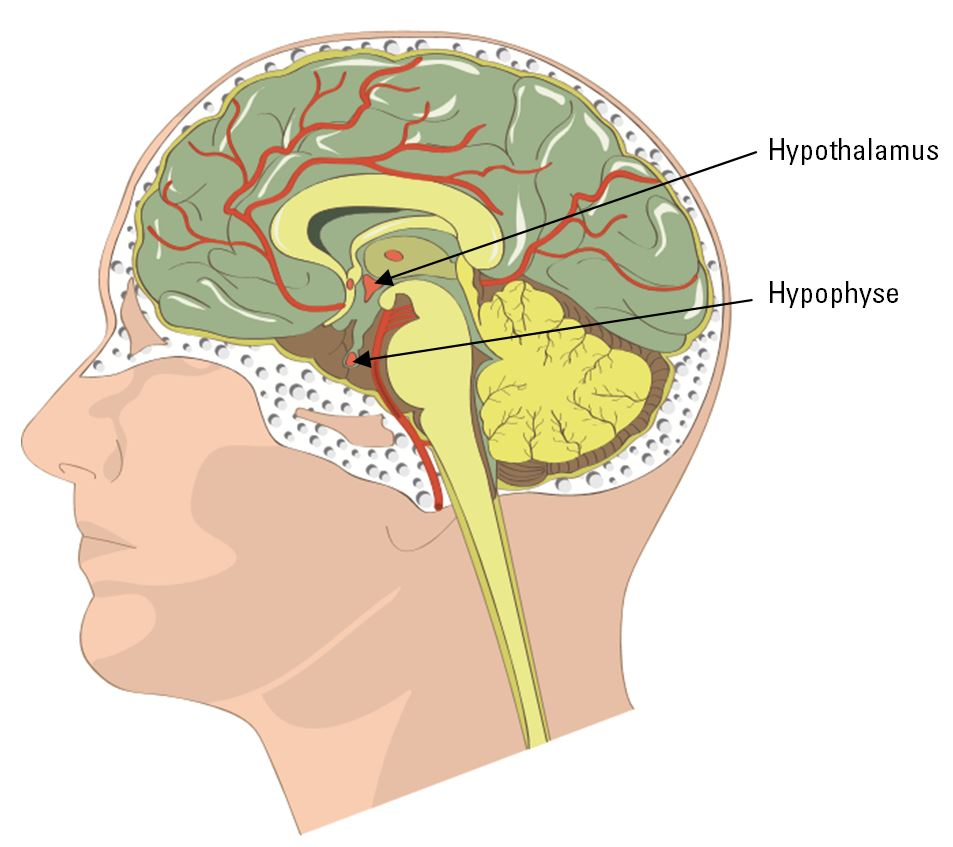
\includegraphics[scale=0.17]{cerv.jpg}
\captionof{figure}{Schéma du cerveau reprsentant le complexe hypothalamo-hypophysaire\tss{\cite{complexe}}}
\end{center}

\begin{itemize}
\item Améliorer l'armée : dans ce domaine environ 1 soldat sur 20 meurt durant des séries d'entrainement. La réalité virtuelle a intégré l'armée et grâce à cette révolution les militaires sont capables de se former dans un environnement en toute sécurité. Mais cette technologie est surtout utilisée dans les simulateurs de vol.

\item Faire du shopping : la réalité virtuelle va intervenir dans le commerce et va rendre ceci plus interactif. Les clients auront la possibilité de se promener dans les boutiques comme s'ils y étaient. Certain scientifique cherchent  même une application qui permettrait de scanner nos corps afin d'essayer des vêtements à distance.(mettre décathlon citations). Pour la marque Décathlon, la réalité virtuelle a surtout permis un gain de place et une meilleure promotion pour leur produit : les tentes Quechua. ``Aujourd'hui, la gamme étant composée de quatorze modèles allant de deux à huit places, il ne faudrait pas moins de 500\,m\tss{2} de surface pour pouvoir exposer tous les modèles et permettre à l'acheteur de comparer différents produits pour trouver la tente idéale'', explique l'enseigne de sport dans un communiqué.

\item Simulateur de conduite : depuis quelques années certaines écoles de conduite proposent des cours de conduite en salle sur des simulateurs. Ce sont de grosses machines qui sont très intéressantes pour des élèves en apprentissage de conduite. Ils peuvent travailler des points comme les démarrages/arrêts ainsi que les changements de vitesse et leur tenue au volant, et aussi comment éviter les premières erreurs. C'est donc un stress qui leur est enlevé.\\
Cependant leur utilisation ne doit pas dépasser les 5 à 10\,h car il y a quand même une grosse différence entre des machines de réalité virtuelle de conduite et les sensations d'une vraies voiture dans un environnement non virtuel.
Le but de ces simulateurs de conduite est de placer le conducteur dans un environnement comparable à celui d'une conduite réelle mais où l'environnement et le véhicule sont totalement représentés par des modèles logiciels.
\begin{center}
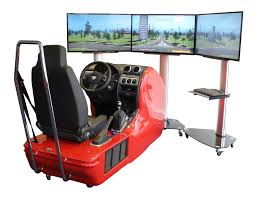
\includegraphics[scale=0.75]{onduite.jpg}
\captionof{figure}{Exemple de simulateur de conduite\tss{\cite{conduite}}}
\end{center}

\item Simulateur de vol : contrairement à ce qu'on peut imaginer ce sont les simulateurs de vol qui utilisent le plus la VR.
Ces simulateurs peuvent être utilisés pour le développement d'aéronefs, l'entrainement des équipages aux fonctions de bord (pilotage, navigation\ldots{}). Tout cela permet aux personnes qui l'utilisent d'apprendre, de s'améliorer \ldots{} Ce dispositif est de plus en plus répandu dans ce type de profession.
\begin{center}
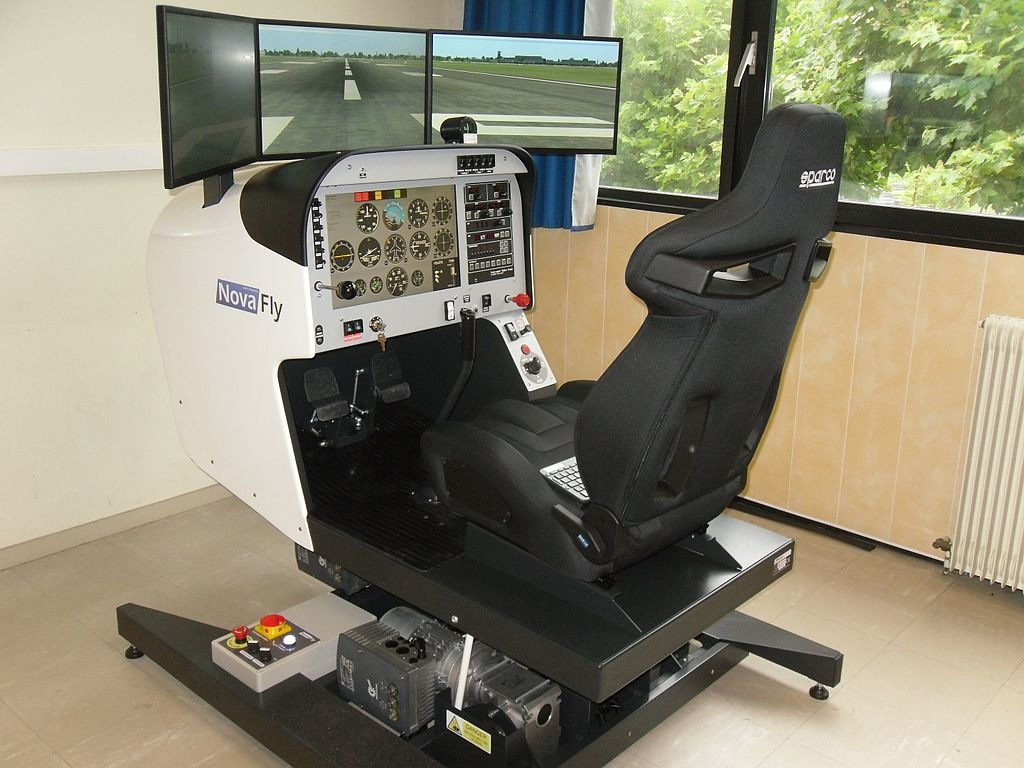
\includegraphics[scale=0.25]{conduite.jpg}
\captionof{figure}{Exemple d'un simulateur de vol\tss{\cite{vol}}}
\end{center}
\end{itemize}
\section[Peur et réalité virtuelle]{Combat et thérapie par la peur}

De nos jours, il existe de nombreux traitements pour les troubles ou les phobie grâce au développement de la technologie numérique comme la réalité virtuelle.
Comme nous l'informe l'expert Eric Malbos,  la réalité virtuelle recommande le traitement des troubles anxieux, qui comporte les phobies mais également le troubles obsessionnels. On l'adopte aussi dans le cas du stress post-traumatique (en cours d'expérimentation dans un centre hospitalier). Cette méthode aide a l'arrêt du tabac qui est nocif pour la santé et l'environnement.

Le principe de la thérapie par la réalité virtuelle se déroule avec de nombreuses séances. En effet le patient n'est pas plongé immédiatement en réalité virtuelle. Pour commencer, ont détermine avec notre patient les problèmes exacts du type de phobie, de troubles ou le degré de son anxiété. Afin de commencer, nous lui apprenons des techniques de relaxation et de respiration qui lui seront utile pour gérer sa réaction face à ses peurs. Plonger une personne qui n'a pas suivit ce traitement anticipé, serait non productif et va placer le patient dans un état de panique plus avancé.

Par la suite, le patient est exposé à la réalité virtuelle pour combattre sa phobie ou son trouble préalablement défini auparavant. Les paramètres sont controlés de facçn douce et progressive de manière que le patient soit à laise et décontracté. Par exemple, pour un phobique de l'avion, les possibilités d'expositions sont multiples. Un avion en réalité virtuelle peut être plein, à moitié plein, vide\ldots{}  Si la personne a besoin de rentrer et sortir de l'avion, c'est possible, de même pour celles qui ont peur du décollage.. \'{E}galement pour quelqu'un qui a la phobie du sang, ou des araignées, on l'immergera dans un environnement où il sera mis en contact par étapes avec sa peur.



\chapter[Dangers]{Les dangers pour la santé}

\section{Effets sur l'oeil}

A ce stade, cette technologie est assez nouvelle et il est donc difficile d'avoir du recul sur les effets néfastes. Cependant, il y a déjà des hypothèses soumises.

\subsection{Acomodation excessive} Les casques de réalité virtuelle reposent sur l'accomodation des yeux qui réussisent à voir un unique objet alors que l'écran du casque en possède 2 : Le processus d'accomodation vise à modifier la courbure du cristallin dans l'oeil par le biais des muscles ciliaires pour permettre une vision nette même lorque les objets sont très proches.
D'où l'hypothèse des médeicin: utiliser cette nouvelle  technologie a très longue durée peut favoriser la perte de capacités d'accomodation et ainsi favoriser l'apparition de dommages au niveau de la vue et rendre nécessaire des moyens de correction de la vue comme des lunettes, des lentilles ou la chirurgie.

\subsection{La lumière bleue, à ne pas négliger ?}

Depuis quelques mois, un scientifique a récemment partagé ses inquiétudes concernant un autre risque encouru par les utilisateurs de la réalité virtuelle : celui d'abimer irréversiblement la rétine, à cause de la lumière bleue.

L'apparition des nouveaux écrans ``OLED'' sur la plupart des nouvelles technologies comme les smartphones, quelques télévisions mais pratiquement tous les casques de la réalité virtuelle poussent les scentifiques  à se poser des questions fondamentales sur les dangers potentiels de certaines lumières.

Un téléviseur dit  LCD  est composé d'une LED par pixel ce qui nous donne ce schéma :

\begin{center}
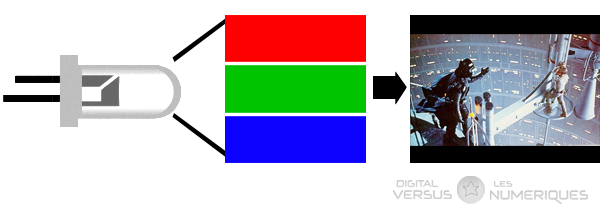
\includegraphics[scale=0.5]{led.jpg}
\captionof{figure}{Composition d'un pixel d'un écran LED\tss{\cite{led}}}
\end{center}


Pour un écran OLED, il y a trois diodes pour chaque pixel, ce qui nous donne ce schéma :

\begin{center}
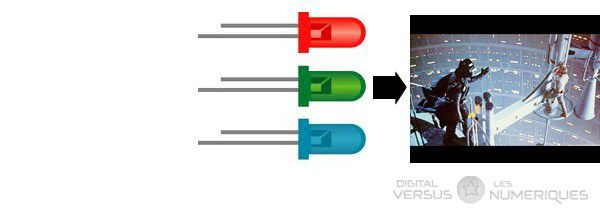
\includegraphics[scale=0.5]{oled.jpg}
\captionof{figure}{Composition d'un pixel d'un écran LED\tss{\cite{led}}}
\end{center}

Dans ces appareils, chaque pixel représente 3 LED capable d'émettre n'importe quelle couleur. Or certaines teintes de bleu de longueur d'ondes 415 à 450 nanomètres semblent être nocives pour les yeux.

Si on cherche à savoir pourquoi c'est ces longueur d'ondes précisement qui semblent visées, il faut définir ce qu'est une radiation lumineuse. Une radiation lumineuse peut être décrite comme une onde ou comme une particule appelée photon. Cette particule se déplace à la vitesse de la lumière et ne possède ni masse, ni charge. L'énergie d'un photon est définie par la formule :
\begin{center}
 \Large{$\Delta E = \frac{h \times c}{\lambda}$}
\end{center}
 Avec $\Delta E$ le quantum d'énergie en $\mrm{J}$, $h$ la constante de Planck en $\mrm{J \cdot s^{-1}}$ et $c$ la célérité en $\mrm{m \cdot s^{-1}}$ ainsi que $\lambda$ en $\mrm{m}$. Or si on détermine le quantum d'énergie des longueurs d'ondes de $415$ à $450$ nanomètres, on obtient :
\[
\begin{array}{rcccl}
\Delta E_1 &=& \dfrac{6{,}63 \cdot 10^{-34} \times 3,0 \cdot 10^8}{415 \cdot 10^{-9}} &=& 4{,}79 \cdot 10^{-19}\u{J} \\

&&&&\\

\Delta E_2 &=& \dfrac{6{,}63 \cdot 10^{-34} \times 3,0 \cdot 10^8}{450 \cdot 10^{-9}} &=& 4{,}42 \cdot 10^{-19}\u{J}
\end{array}
\]

On obtient donc des valeurs comprises entre $ 4{,}42 \cdot 10^{-19}\u{J}$ et $4{,}79 \cdot 10^{-19}\u{J}$.

Or si on compare nos résultats au quantum d'énergie émis par un photon correspondant à une longueur d'onde proche de $700$ nanomètres(rouge), on obtient:
\begin{center}

\[
\Delta E_3 = \dfrac{6{,}63 \cdot 10^{-34} \times 3,0 \cdot 10^8}{700 \cdot 10^{-9}} = 2{,}84 \cdot 10^{-19}\u{J}
\]

\end{center}

On peut donc voir que le quantum d'énergie délivré par le photon responsable de la couleur rouge est une fois et demi inférieur à celui de la lumière bleue.
C'est donc pourquoi une si grande quantité d'énergie inquiète les scientifiques face aux répercutions possibles sur la rétine puisque la lumière est réfractée successivement dans l'\oe{}il jusqu'à toucher la rétine. Les hypothèses disent que ces ondes lumineuses particulières peuvent détruire les cellules de la rétine ainsi que de la fovéa.

La réalité virtuelle ne fait donc pas vraiment bon ménage avec les yeux. Mais pas de quoi s'en inquiéter outre-mesure, disent les médecins. Il suffit de faire preuve de bon sens : ne pas laisser les enfants utiliser ces casques sans surveillance, faire des pauses régulières pour reposer les yeux, et bien essayer le matériel avant de l'acheter.

\section{Effets sur l'équilibre}

En temps normal, le cerveau utilise trois sources de données pour informer l'organisme sur sa position et ses mouvements : l'oreille interne, les muscles et les yeux. Mais une fois le casque sur la tête, les yeux indiquent que vous êtes dans un grand huit, mais l'oreille interne et les muscles disent que ce n'est pas le cas : cette incohérence des informations sensorielles peut provoquer des nausées.\\
 La plus importante est l'incohérence entre la vision et  l'organe de l'équilibre. L'utilisateur voit un mouvement alors que son corps reste dans un état statique. Le cerveau est perturbé et finit par envoyer des signaux d'alarmes, sous la forme de nausée. La sensation est similaire à celle ressentie par une personne malade en voiture.

L'oreille interne est la partie de notre corps qui assure l'équilibre ; ce role est plus précisément assuré par un organe sensoriel, l'appareil vestibulaire :
il détermine la position de la tête dans l'espace, informe le cerveau de ses mouvements ; il nous permet d'adapter notre position, en coordonnant les mouvements du tronc, du cou, de la tête et la position des yeux.

L'oreille interne est composée d'un réseau de cavités rigides creusées dans l'os temporal. Le vestibule, partie molle dans le l'os temporal est composé de sacs,  l'utricule  et  la Saccule,  mais aussi de trois canaux en demi-cercles, placés à la perpendiculaire les uns des autres, qui contiennent un liquide, l'endolymphe. En fonction des mouvements effectués par la tête, l'endolymphe s'y déplace dans un sens donné et cette information est captée par des récepteurs spécialisés, qui l'envoient au cervelet via le nerf vestibulaire.

Comme ce liquide, bougeant dans ces canaux de facon différente du mouvement, provoque une confusion des informations qui parviennent au cerveau et ce dernier envoi un signal d'alarme, la sensation de nausée apparait donc.
Au niveau de la réalité virtuelle, nous avons recueillit le témoignage de Franck Petriz, récemment diplomé de l'école Epitech Nancy,qui a réalisé un logiciel de simulateur de conduite, a remarqué, pour neutraliser cet effet ou le diminuer, il fallait placer au niveau de l'écran, un triangle noir statique, qui recrée l'absence d'image au niveau du nez.

\begin{center}
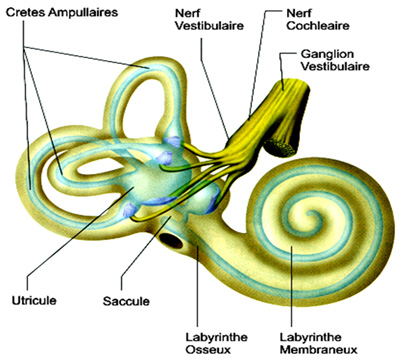
\includegraphics[scale=0.5]{oreille.jpg}
\captionof{figure}{Schéma de l'oreille\tss{\cite{oreille}}}
\end{center}

\section[Cerveau]{Effets potentiels sur le cerveau}

Le professeur Mayank Mehta de la célèbrniversité UCLA en Californie, étudie depuis 2009 les effets de la réalité virtuelle sur les neurones. Une expérience menée sur des rats placés dans un univers virtuel montre que 60\,\% des neurones de l'hippocampe, partie du cerveau dédiée à la mémoire et aux repères spatiaux, devenaient inactifs et que les 40\,\% restant fonctionnaient de facon chaotique. Le professeur a également noté une baisse sensible au niveau de l'activité électrique de tous les neurones. Même si l'étude a seulement été réalisée sur des rats, ses résultats peuvent être appliqués à l'homme. Le professeur et son équipe travaillent d'ailleurs actuellement sur une technologie qui leur permettra de comprendre ce qu'il se passe à l'intérieur d'un neurone chez un sujet placé dans un univers virtuel. Si la réalité virtuelle peut donc être utilisée pour  traiter, son influence sur les neurones n'est pas non plus à négliger.

Alors même si les effets éventuels de la VR sur la santé ne seront connus que dans quelques années, voici quelques consignes simples pour  s'en protéger. Tout d'abord, il convient d'interdire la VR aux enfants de moins de 12 ans, leur système visuel et cerveau n'étant pas complètement mature. Il est également nécessaire de faire des pauses toutes les 15 à 20 minutes, comme le rappellent les fabricants de casques VR. Et même si le besoin ne s'en fait pas ressentir, il est aussi fortement déconseillé de prendre le volant après une session VR et enfin en cas d'inconfort même minime, il faut immédiatement arrêter l'expérience.

Il nous est donc impossible de savoir les conséquences de la réalité virtuelle sur le cerveau. Nous savons par contre qu'elle apporte beaucoup de bienfaits médicaux dans divers domaines. Ces aspects négatifs n'ont pas encore été révélés et il convient donc d'être prudent et de suivre les études menées pour connaitre les véritables conséquences de la réalité virtuelle sur le cerveau et l'organisme.

Cependant, une utilisation trop importante de la réalité virtuelle, associé à des jeux violents, plus un comportement instable peu favoriser la confusion et l'agressivité chez certaines personnes.

\vspace{2cm}
\section{Conclusion}




.........................

\vspace{9cm}





















........................


\section*{Remerciements}

Nous voulons remercier de nombreuses personnes sans qui nous n'aurions pu réaliser ce travail.

Tout d'abord, nous remercions notre professeur référent M. \sc{Julian} qui nous a suivi et conseillé durant tout notre projet, ainsi que tous les autres profeseurs de TPE et de l'établissement qui ont pu nous apporter leur aide.

Nous remercions aussi tous les élèves de l'établissement Arthur \sc{Varoquaux} qui ont pris sur leur temps pour répondre à notre sondage et qui nous ont permis de récolter toutes ces données.

Nous remercions l'Ecole Epitech pour avoir apporté ds réponses à nos questions.

Nous voulons remercier spécialement l'entreprise Human Games qui nous a très chaleureusement acueilli et qui nous a permis d'expérimenter la réalité virtuelle mais aussi pour tous leurs précieux conseils qui nous ont vraiment permis de structurer et d'apporter des précisions à notre récit. Sans eux, nous n'aurions pas pu mesurer réellement les enjeux de cette nouvelle technologie.

Enfin, nous remercions tous nos proches pour avoir pris de eur tems pour relire et nous conseiller sur ce rapport.



{\color{white} \cite{1, 2, 3, 4, 5, 6, 7, 8, 9, 10, 11, 12, 13, 14}}

\appendix{}

\listoffigures{}

\printbibliography{}































%%%%%%%%%%%%%%%%%%%%%%%%%%%%%%%%%%%%%%%%%%%%%%%%%%%%%%%%%%%%%%%%%%%%%%%%%%%%%%%

\end{document}